\documentclass[11pt]{article}
\usepackage[margin=1in]{geometry}
\usepackage{amsmath,amssymb}
\usepackage{graphicx}
\usepackage{booktabs}
\usepackage{array}
\usepackage{xcolor}
\usepackage[numbers,round]{natbib}
\usepackage[colorlinks=true,linkcolor=blue!50!black,citecolor=blue!50!black,urlcolor=blue!50!black]{hyperref}
\newcolumntype{L}[1]{>{\raggedright\arraybackslash}p{#1}}
\graphicspath{{figs/}}
\makeatletter\g@addto@macro\UrlBreaks{\do\-}\makeatother

\title{ExoHominid: A Human Connectome-Structured Reservoir Policy for Robot Learning\thanks{Preprint, not peer reviewed. Code and project page to be released.}}
\author{Jude Onyenze\\
Department of Mechanical Engineering, University of Texas at Dallas\\
Richardson, Texas, USA\\
\href{mailto:chisimdi.onyenze@utdallas.edu}{chisimdi.onyenze@utdallas.edu}\\
ORCID: \href{https://orcid.org/0009-0000-1418-1058}{0009-0000-1418-1058}}
\date{}

\begin{document}
\maketitle

\begin{figure}[!h]
  \centering
  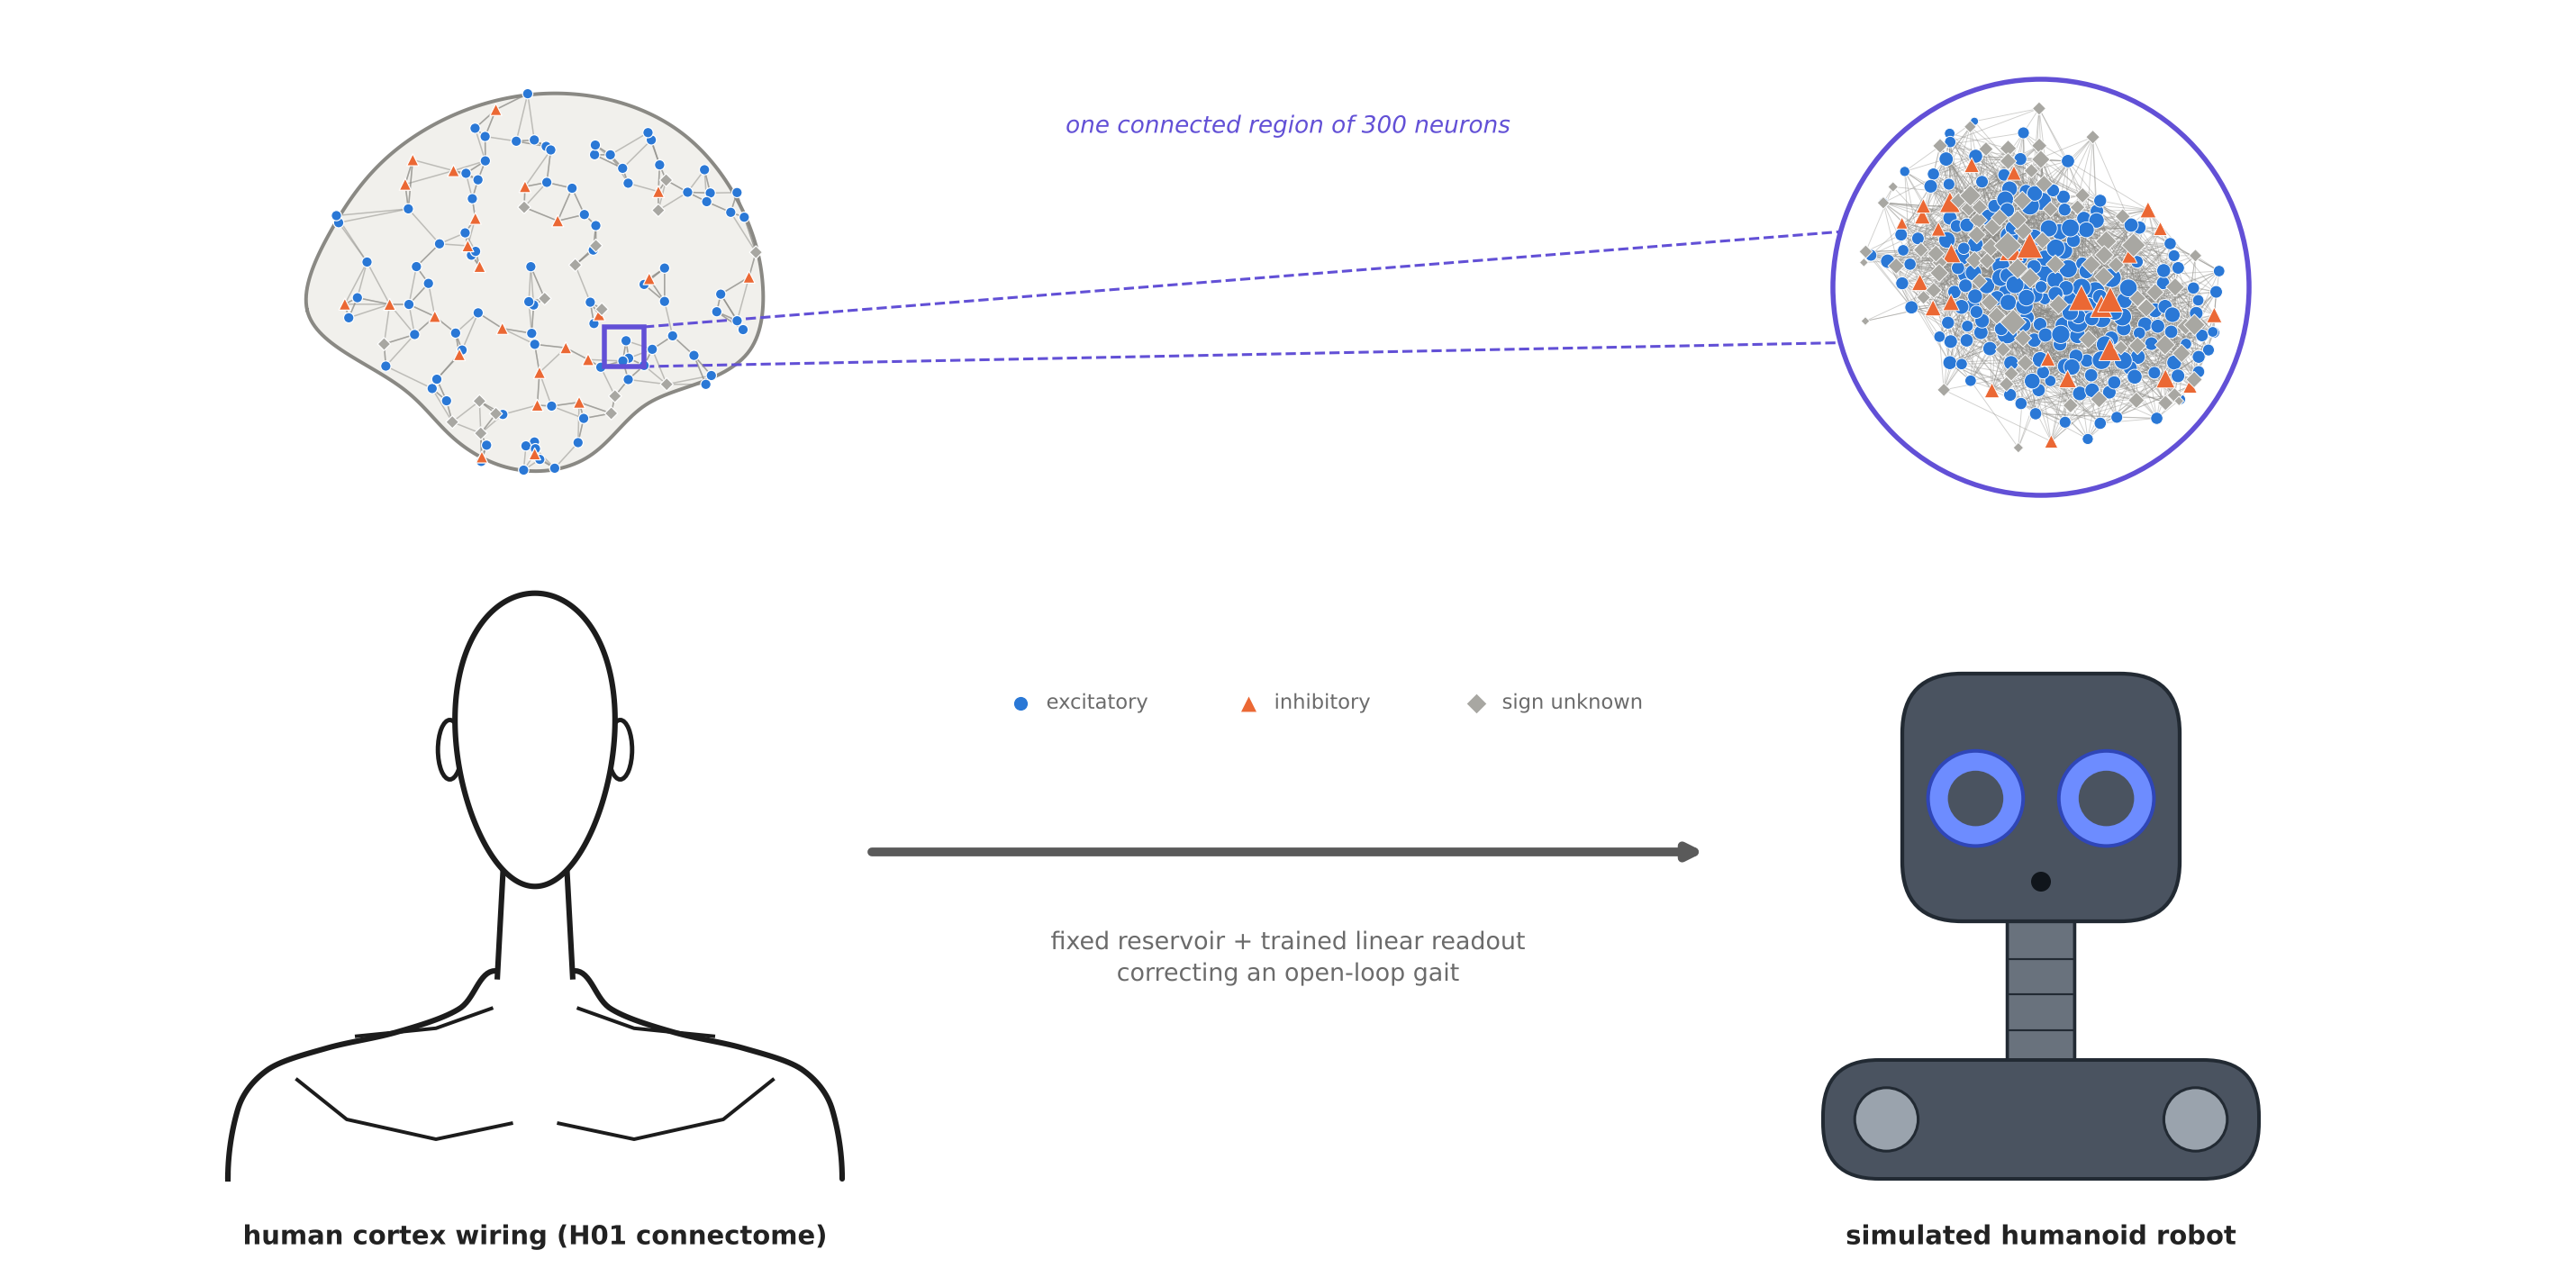
\includegraphics[width=0.8\linewidth]{fig_overview.png}
  \caption{Overview. The wiring of a human cortical microcircuit (H01 connectome; the brain network is an illustration) is cut into a connected 300-neuron region, which becomes the fixed recurrent core of the controller of a simulated humanoid robot; only a linear readout on top of it is trained and it corrects an open-loop gait. Circles: excitatory neurons, triangles: inhibitory, diamonds: sign unknown. The human and the robot are schematic drawings.}
  \label{fig:overview}
\end{figure}

\begin{abstract}
Can the wiring of a human cortical microcircuit serve as the recurrent core of a robot controller? To ask this, we took the H01 human temporal cortex connectome \citep{shapsoncoe2024h01}, extracted a directed, signed graph of 16,599 neurons and sampled 300-neuron subgraphs. Each subgraph became the fixed recurrent network of a reservoir whose linear readout adds small corrections to an open-loop gait of a simulated DARwIn-OP pushing a box. We compared it with degree-preserving shuffles, random graphs, a standard echo-state network (ESN), three sign policies, a memoryless linear readout and a constant correction, over three subgraphs and 30 evaluation episodes per subgraph. Trained readouts raised the success rate from 33\% (open loop) to between 60\% and 99\%, depending on the reservoir. With signs randomised, real and shuffled wiring scored 94\% and 97\% ($p=0.7$), and a constant correction with three trained numbers reached 99\%, equal to the best reservoir. This is a very specific task that is easy to train and does not require feedback, so it is not demanding enough to show whether structuring a network on human brain wiring helps; a more complex test would allow a better evaluation. The measured sign assignment lowered performance on one subgraph. We report these results, the controls that accompany them, and a pre-registered protocol for next steps: more refined and more difficult tasks that require adaptation.
\end{abstract}

\section{Introduction and Related Work}
Can the wiring of a real human cortical circuit be used as the recurrent core of a robot controller, and does it do better than wiring that is merely random? This paper tests that question with a deliberately simple design on one specific task, which turned out to be easy to train.

Connectomics has moved quickly in the 2020s. Complete wiring diagrams now exist for the adult fruit fly brain \citep{dorkenwald2024flywire}, and they have been turned into whole-brain computational models \citep{shiu2024fly}. For the human cortex, the H01 dataset \citep{shapsoncoe2024h01} reconstructs one cubic millimetre of left anterior middle temporal gyrus from a 45-year-old patient, with about 57,000 cells and 150 million synapses. Connectome-based reservoir computing has been explored with human, macaque, marmoset and other animal connectomes \citep{suarez2021learning,damicelli2022brain,dandrea2022complex,morra2022imposing,suarez2024conn2res} and, recently, with the fruit fly connectome \citep{costi2025drosophila}, and wiring inspired by the nematode \emph{C.~elegans} has been used to steer a vehicle \citep{lechner2020ncp}. We are not aware of work that drives a simulated humanoid with a synapse-resolution human cortical subgraph and tests it against matched controls, although we have not exhausted the literature.

A reservoir is a fixed recurrent network whose only trained part is a linear readout \citep{jaeger2001esn,lukosevicius2009reservoir}. That makes it a clean way to ask about structure: the wiring is given, training cannot reshape it, and any benefit of a particular graph must come from the graph itself. We therefore built reservoirs from H01 subgraphs (Figure~\ref{fig:nested}) and compared them with controls that keep or destroy specific properties of the wiring.

\begin{figure}[t]
\centering
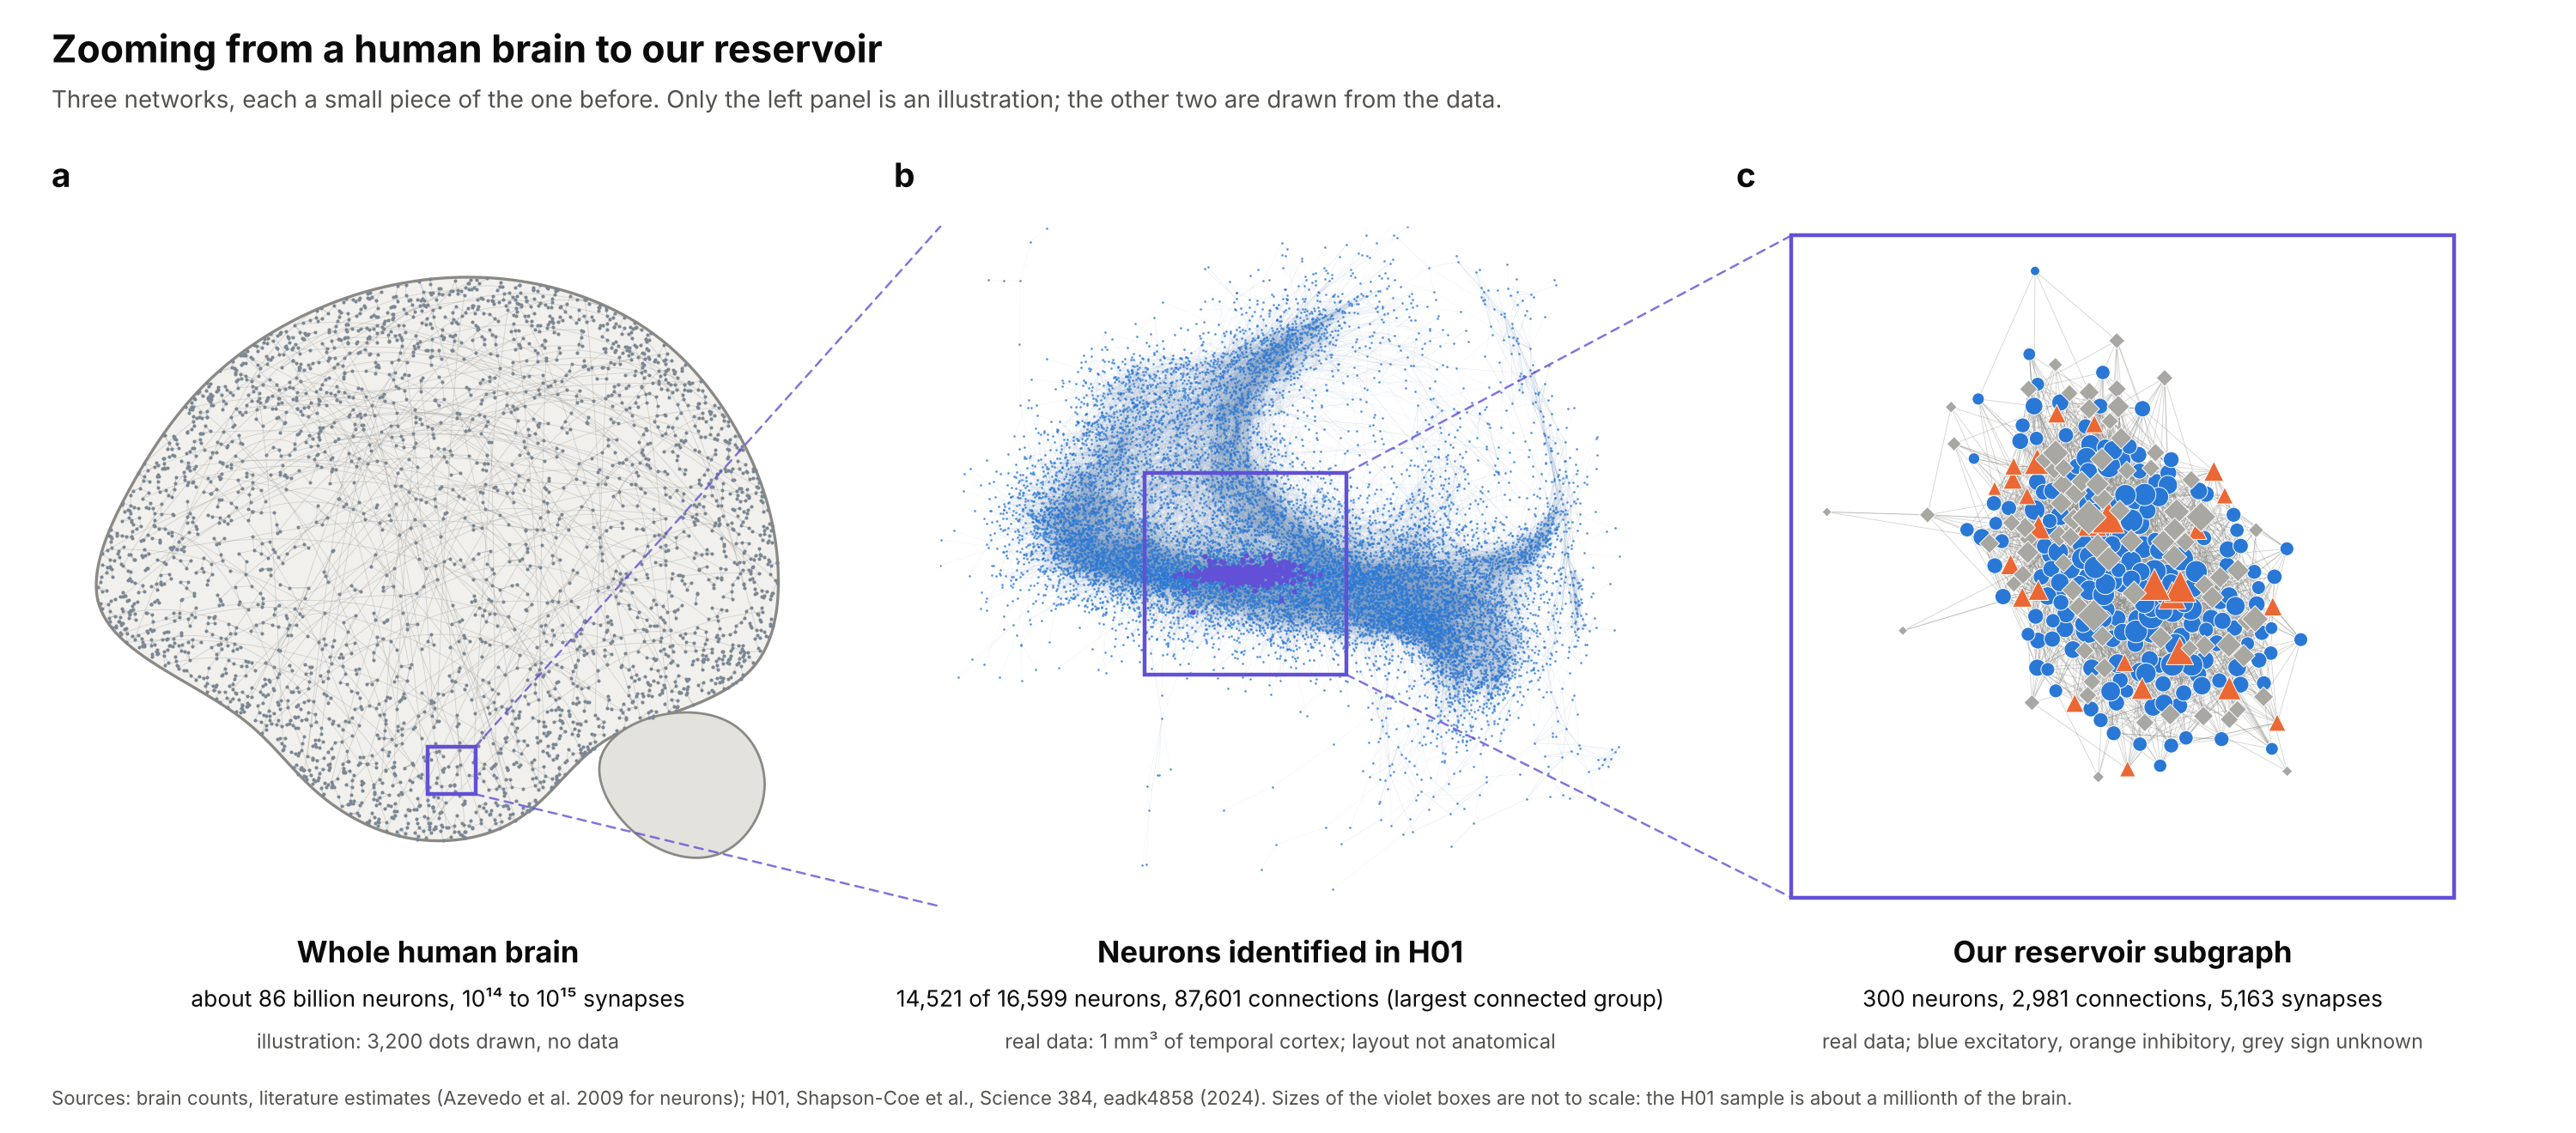
\includegraphics[width=\linewidth]{fig_nested.png}
\caption{From a human brain to our reservoir. The H01 volume is a roughly millionth of the volume of a human brain; the neurons identified in it form a graph, from which we cut a 300-neuron connected region that becomes the reservoir.}
\label{fig:nested}
\end{figure}

Before running the main experiment we wrote down one hypothesis: reservoirs built from real H01 wiring with measured excitatory and inhibitory signs reach a higher success rate than each of four controls (degree-preserving shuffle, random graph, standard ESN, H01 wiring with permuted signs). On this task the hypothesis was not supported, and the controls show why the task is too easy to test it well. Our contributions are:
\begin{itemize}
\item an open pipeline from the H01 synapse tables to signed neuron graphs and 100-, 300- and 1,000-neuron subgraphs;
\item a robot benchmark with matched controls, including two controls that have no reservoir at all;
\item the finding that a constant three-number correction solves our final task, so a more demanding task is needed to compare networks;
\item a record of the problems that shaped the protocol: an untuned open-loop baseline, an unstable trainer, a ceiling effect, and a broken simulator state.
\end{itemize}

\subsection{Related Work}
Three lines of work are closest to ours, and none of them tests human cortical wiring against matched controls on a robot task. First, \emph{connectomes as reservoirs}: Suárez and colleagues built echo-state networks from human diffusion-MRI connectomes and showed that performance depends on topology and dynamics \citep{suarez2021learning}, and released the conn2res toolbox for this purpose \citep{suarez2024conn2res}. Damicelli and colleagues found that macaque, marmoset and human connectomes perform about as well as randomly wired reservoirs when connection strengths stay sufficiently random \citep{damicelli2022brain}; d'Andrea and colleagues compared 45 connectomes from eight species with null models \citep{dandrea2022complex}; Morra and Daley imposed connectome topology on an echo-state network \citep{morra2022imposing}; and Costi and colleagues used the fruit fly connectome as a reservoir for time-series prediction \citep{costi2025drosophila}. These studies work at region or whole-brain scale, or on prediction tasks, whereas we use synapse-resolution cortical wiring with signs on an embodied task. Second, \emph{connectome-inspired control}: neural circuit policies \citep{lechner2020ncp} wire neurons after the \emph{C.~elegans} nervous system for vehicle control. Third, \emph{connectome-constrained and whole-connectome models}: the FlyWire adult fly brain wiring diagram \citep{dorkenwald2024flywire}, a leaky integrate-and-fire model built from it \citep{shiu2024fly}, connectome-constrained networks that predict neural activity in the fly visual system \citep{lappalainen2024connectome} and a physics-based whole-body fly model for locomotion \citep{vaxenburg2025whole} show what connectomes can predict and how they could one day drive a body; a recent report surveys the field \citep{brainemulation2025}. Our data come from H01 \citep{shapsoncoe2024h01}, reconstructed with flood-filling-network segmentation \citep{januszewski2018ffn} developed by Google Research. This list is incomplete: before posting we will add the hemibrain, MICrONS and \emph{C.~elegans} connectome papers.

\section{Method}
We built a graph from the H01 synapse tables, sampled connected subgraphs, used each as a fixed reservoir, trained only a linear readout in simulation, and compared against controls under a protocol written down in advance (Figure~\ref{fig:overview}).

\subsection{H01 Graph}
Figure~\ref{fig:h01pipeline} summarises how the published data become our reservoir. We read the 166 Avro shards of the H01 c3 agglomeration synapse tables, 160,259,769 rows in total. The H01 paper reports 149,871,669 synapses; our export contains somewhat more rows than that count, and we use row counts as edge weights, not as corrected synapse numbers. A cell counted as a neuron if it had at least 5 soma-labelled rows and at least 20 rows as a dendritic receiver, which gave 16,599 neurons. Among them, 87,706 directed connections (148,140 synapse rows, 0.09\% of all rows) link neurons to neurons; 14,683 neurons have at least one such connection, 14,521 sit in the largest connected group, and a giant strongly connected core holds 10,133.

\begin{figure}[t]
\centering
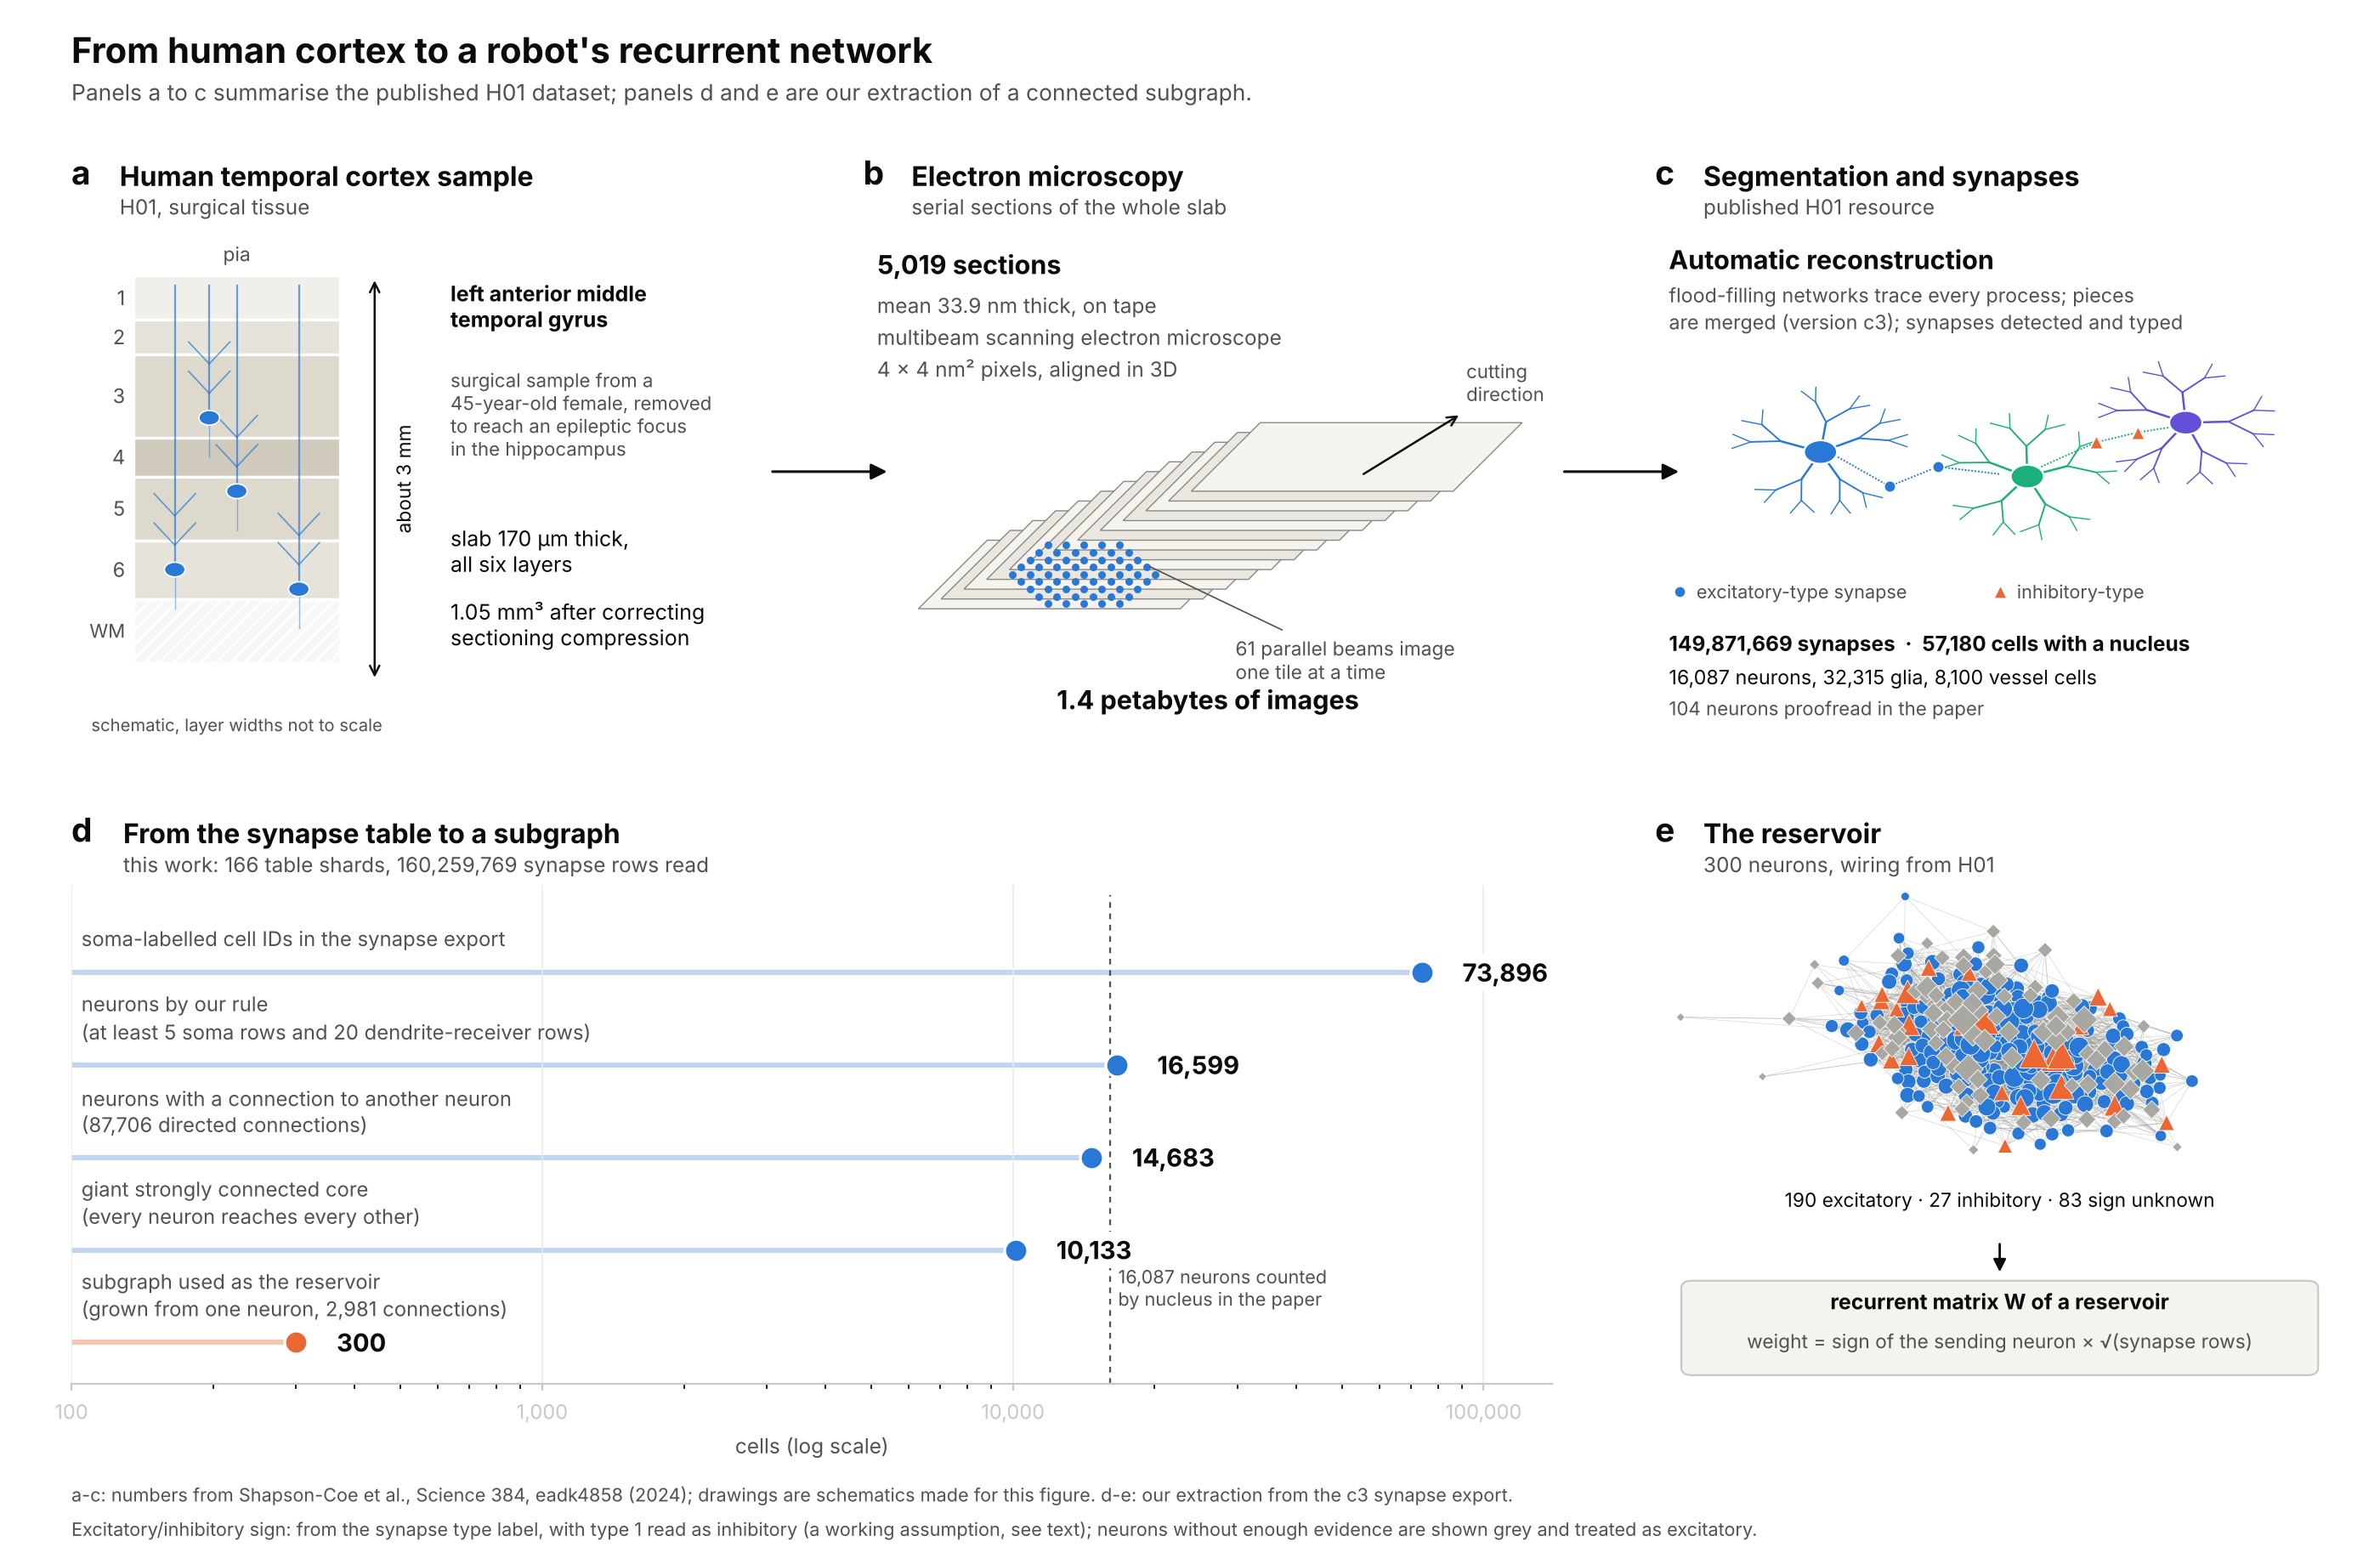
\includegraphics[width=\linewidth]{fig_pipeline.png}
\caption{From the published dataset to a reservoir. Panels a--c summarise H01 (surgical sample, serial-section electron microscopy, automatic segmentation and synapse detection). Panels d and e are our extraction: 166 table shards and 160,259,769 synapse rows give 16,599 neurons by our rule, 87,706 directed connections, a giant strongly connected core of 10,133, and a 300-neuron subgraph used as the recurrent matrix of a reservoir.}
\label{fig:h01pipeline}
\end{figure}

\subsection{Excitatory and Inhibitory Signs}
A synapse either pushes the receiving neuron up (excitatory) or down (inhibitory); in a reservoir this becomes the sign of an entry of the recurrent matrix (Figure~\ref{fig:ei}). We read synapse type~1 as inhibitory, which is a working assumption supported by the type mix of axon-to-soma (79.5\% type~1) and axon-to-axon-initial-segment (85.2\%) contacts, but not verified against labelled cells. Following Dale's principle, a neuron takes one sign, from its output synapses. Neurons without evidence are treated as excitatory. In our subgraphs 12.4\%, 16.3\% and 18.8\% of neurons with a data-derived sign are inhibitory, below the 29.1\% interneuron share the H01 paper reports, so inhibition is probably under-represented.

\begin{figure}[t]
\centering
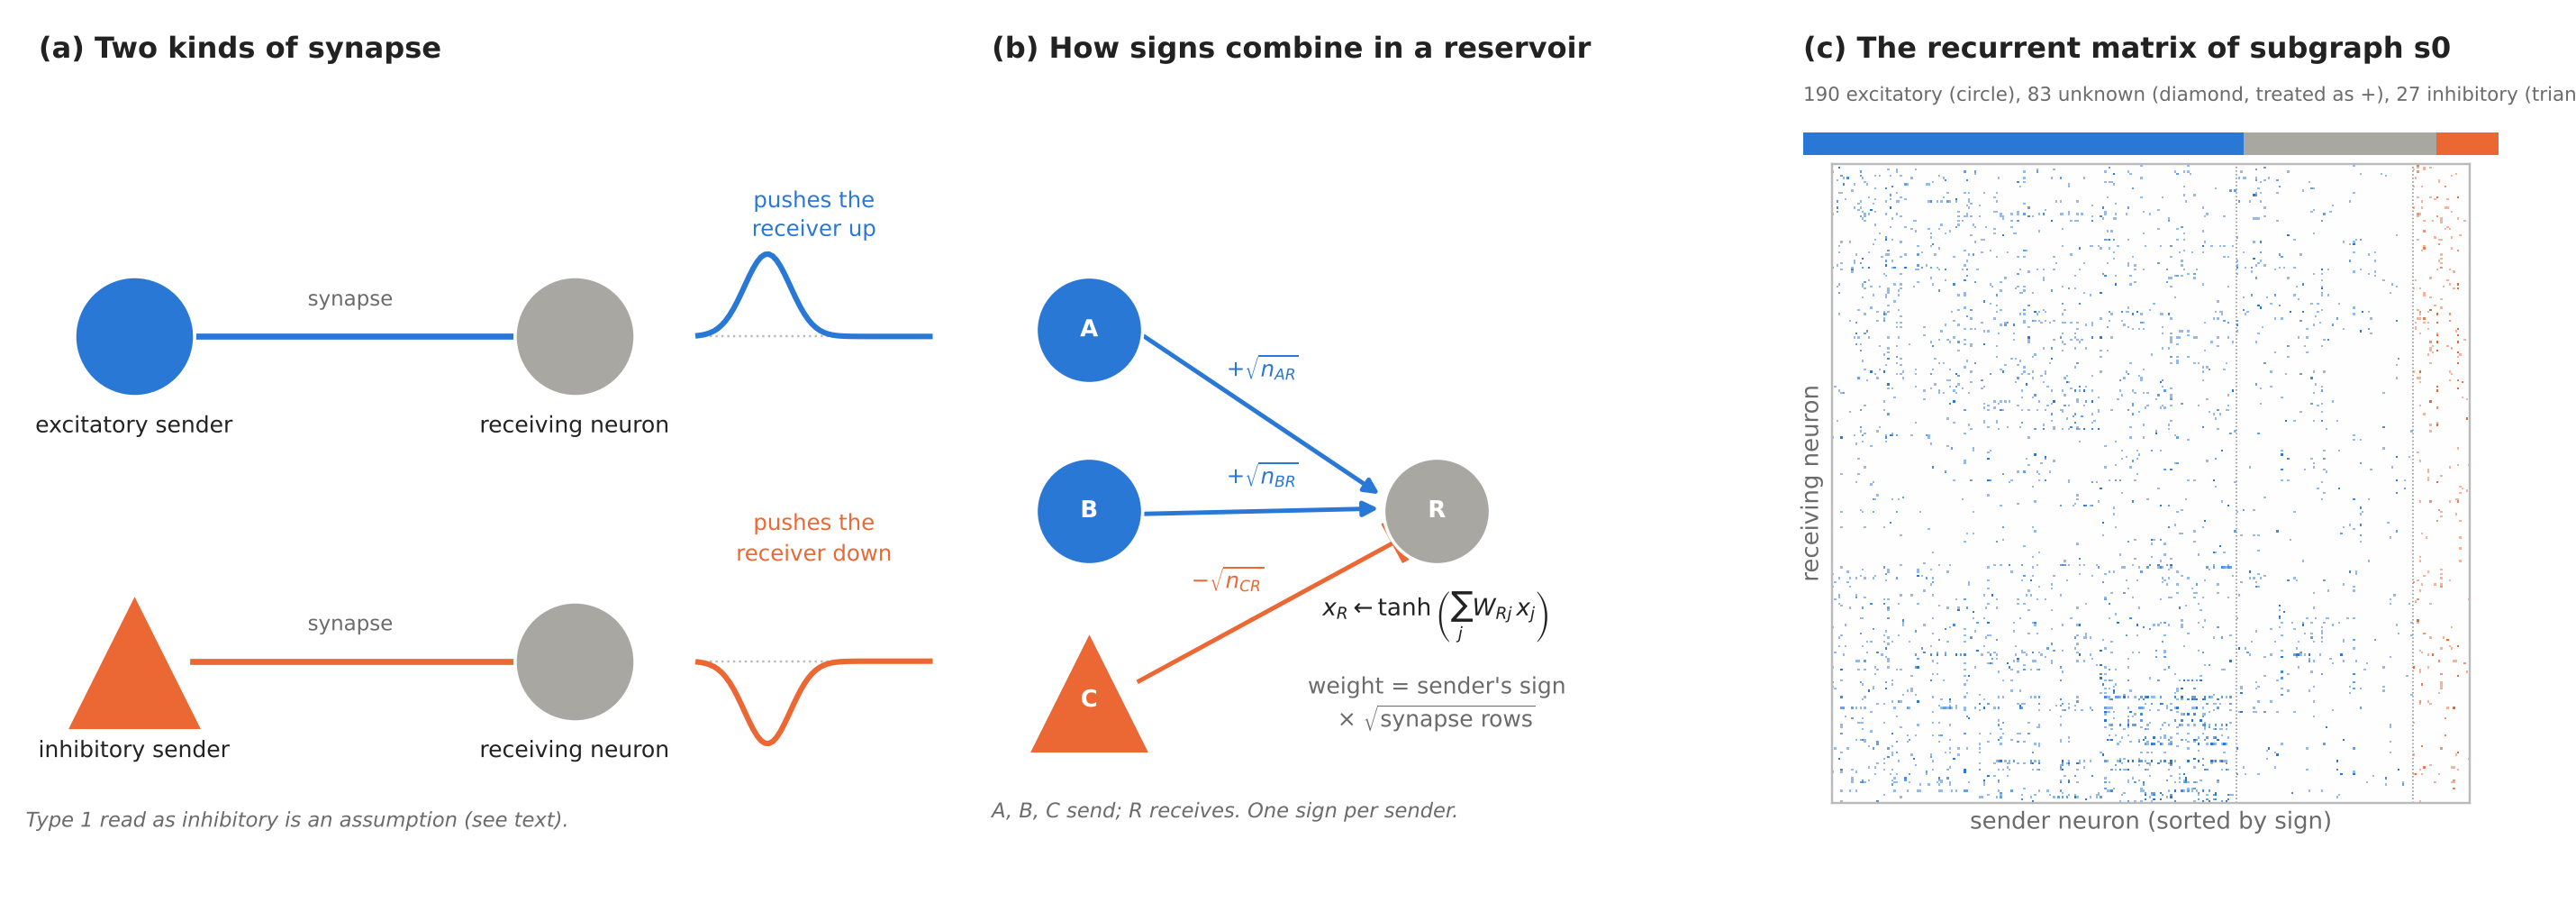
\includegraphics[width=\linewidth]{fig_ei.png}
\caption{Excitatory and inhibitory synapses and how they act inside a subgraph. (a) An excitatory sender (circle) pushes the receiving neuron up, an inhibitory sender (triangle) pushes it down. (b) In the reservoir each connection has weight equal to the sender's sign times the square root of the number of synapse rows, and a receiving neuron sums them before the $\tanh$. (c) The recurrent matrix of subgraph s0 (rows: receivers, columns: senders, sorted by sender sign). Blue entries are excitatory, orange entries inhibitory; senders with no sign evidence (grey bar) are treated as excitatory. Type~1 read as inhibitory is an assumption.}
\label{fig:ei}
\end{figure}

\subsection{Subgraphs}
A subgraph starts at a random neuron in the giant core and grows as one connected region by repeatedly adding the outside neuron most strongly tied to the current set. We used three 300-neuron subgraphs, one per seed (Figure~\ref{fig:subgraphs}). They differ in density, reciprocity and inhibitory share: the third (s2) is the sparsest, has the most reciprocal connections and the most inhibitory neurons.

\begin{figure}[t]
\centering
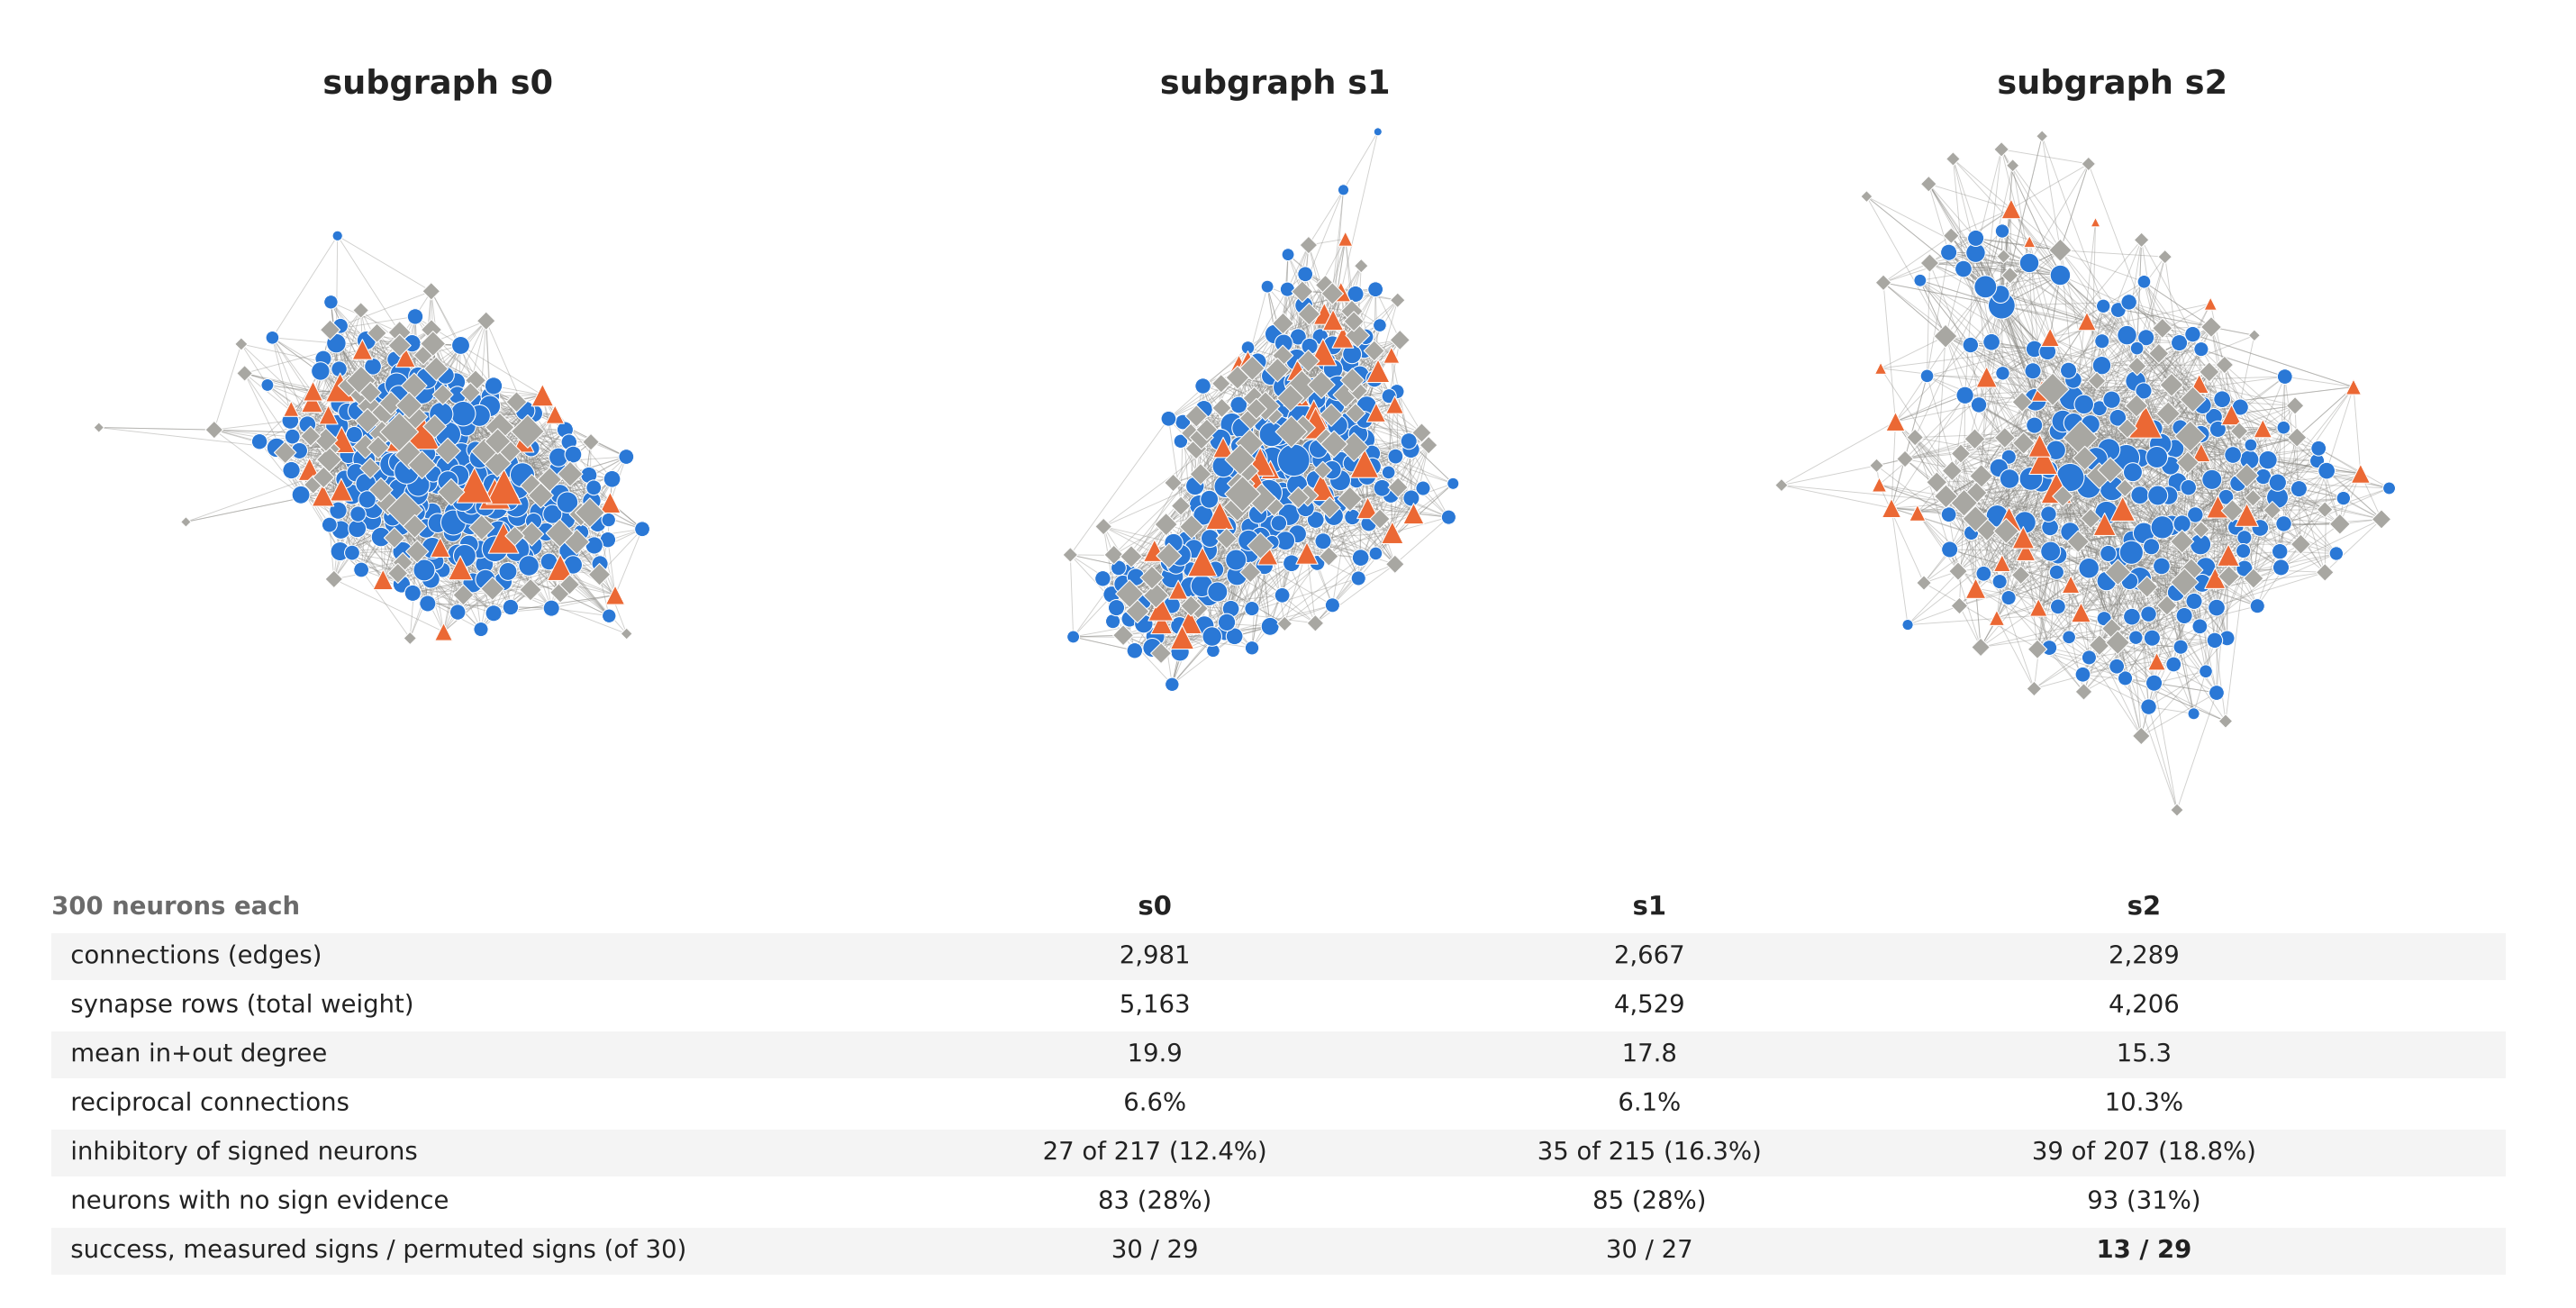
\includegraphics[width=\linewidth]{fig_subgraphs.png}
\caption{The three subgraphs. Excitatory neurons are blue circles, inhibitory neurons orange triangles, and neurons with unknown sign grey diamonds; node size grows with degree. The table lists the structural differences and the final-queue success counts (of 30 episodes) for H01 wiring with measured signs and with permuted signs. The one large drop, 13 of 30 with measured signs on s2, comes with the sparsest wiring and the highest inhibitory share.}
\label{fig:subgraphs}
\end{figure}

\subsection{Reservoir and Policy}
The state follows $x\leftarrow(1-a)\,x+a\tanh(Wx+W_{\text{in}}u)$ with leak $a=0.3$ (Figure~\ref{fig:policy}). Each entry of $W$ is the sender's sign times the square root of the synapse-row count, and $W$ is rescaled to spectral radius 0.9. Input weights are random (25\% of neurons per input, magnitude up to 0.5) and use the same recipe for every graph. The readout is linear with three outputs: a turn command (maximum 0.6 in the walker's own steering parameter), an ankle lean (maximum 0.08~rad) and a stride multiplier ($1\pm0.25$); it has $3\times301=903$ trained numbers. With zero readout weights the policy is exactly the open-loop gait. Inputs are gyroscope (3), accelerometer (3) and gait phase (sine, cosine); the first two queues also gave four simulator-supplied inputs (box gap, box side offset, heading, lateral offset), which the final queue removed.

\begin{figure}[t]
\centering
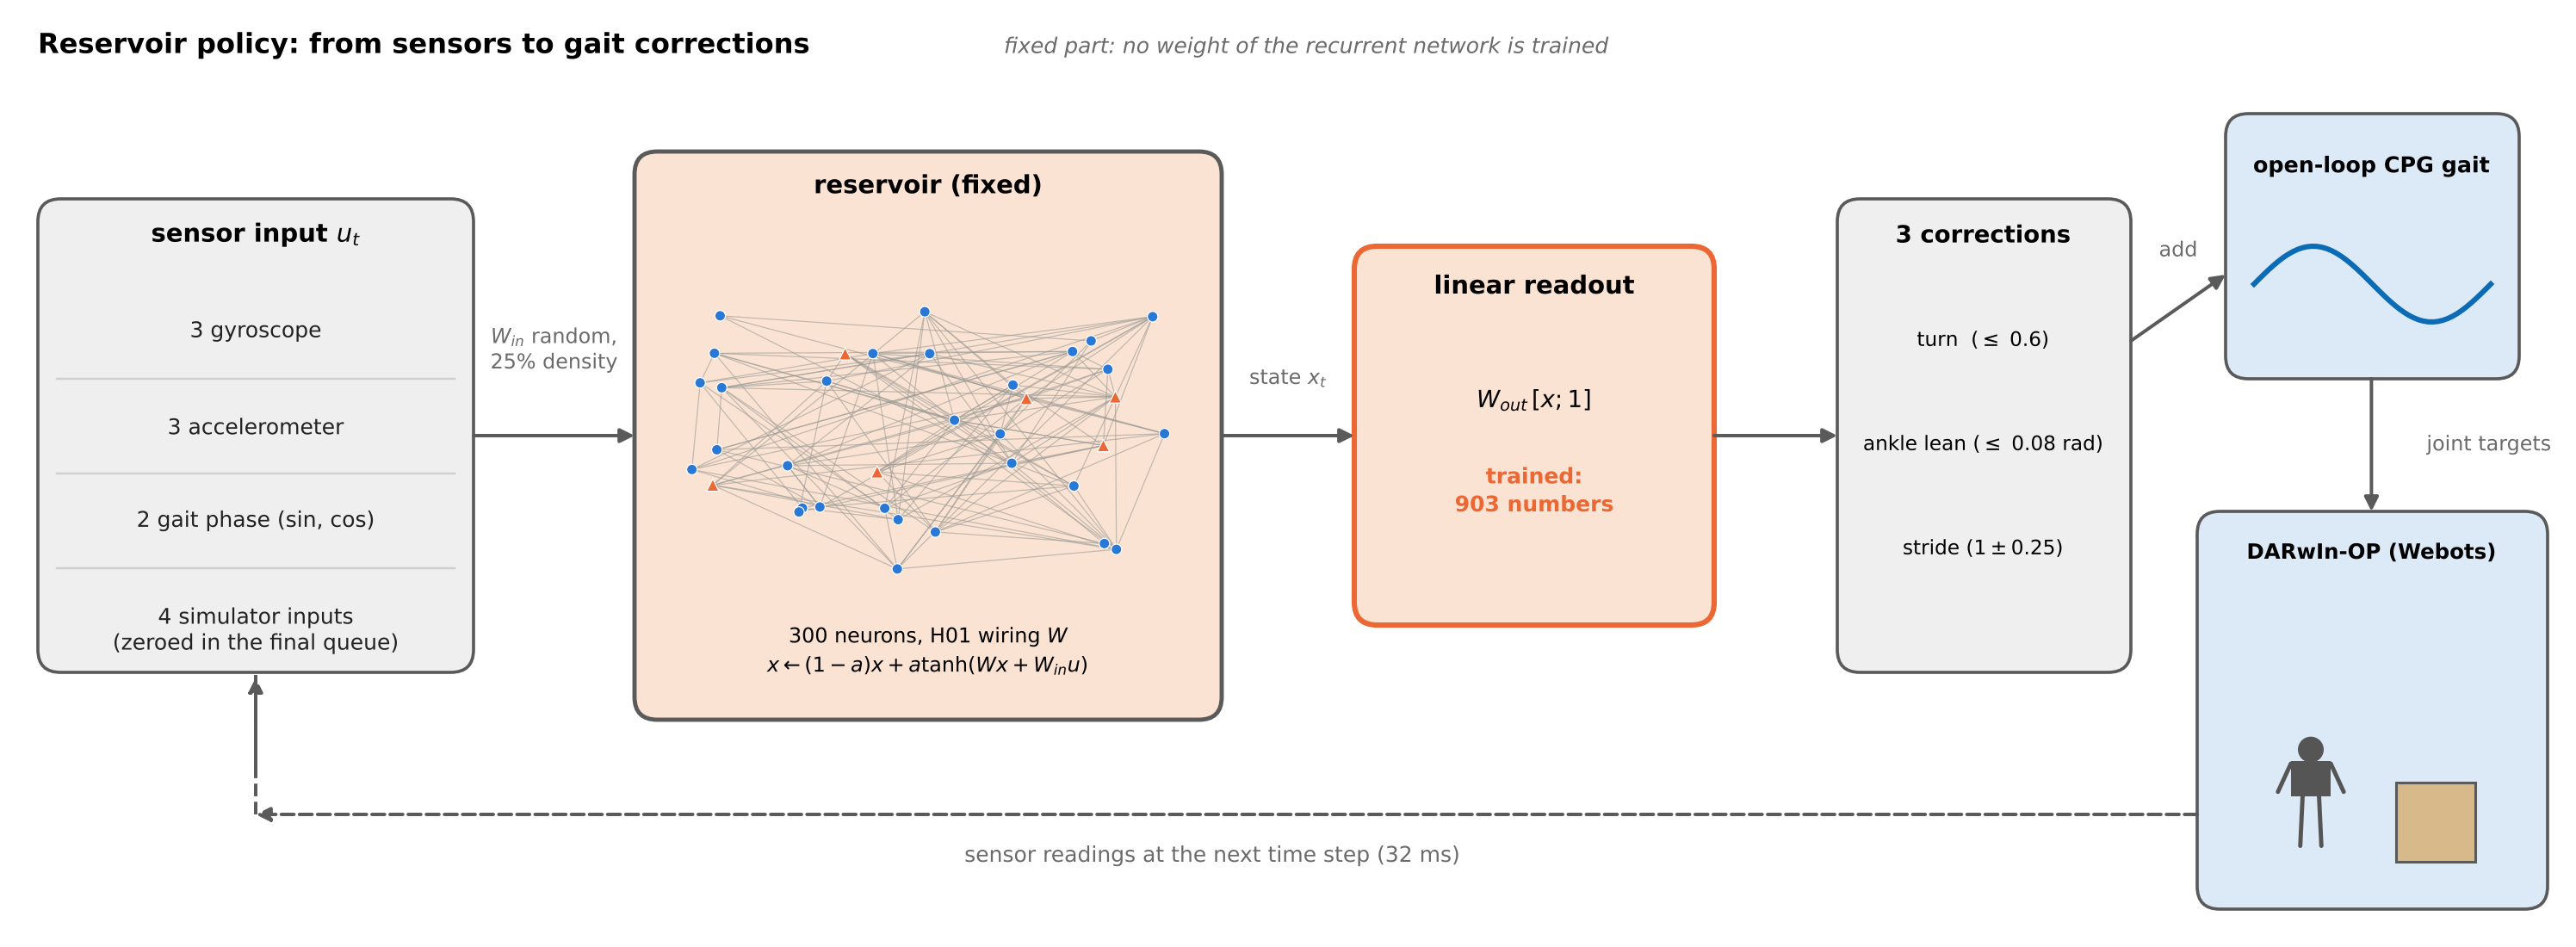
\includegraphics[width=\linewidth]{fig_policy.png}
\caption{The reservoir policy. Sensor readings enter the fixed reservoir through random input weights; a trained linear readout turns the reservoir state into three small corrections that modulate the open-loop gait of the walker; the robot's motion changes the next sensor readings. Only the readout (903 numbers) is trained.}
\label{fig:policy}
\end{figure}

\subsection{Robot and Task}
We evaluate the policy on a pushing task, chosen as a simple test of robot manipulation that also exercises whole-body humanoid motion: a DARwIn-OP \citep{ha2013darwinop} in Webots R2025a \citep{michel2004webots}, with a calibrated open-loop walker, must walk to a 0.6~m cube whose front face starts 0.5~m ahead and push it (Figure~\ref{fig:task}). An episode succeeds when the box has moved 0.40~m. Failure scores combine progress and approach, with penalties for sideways drift, falling and tipping. We evaluate 30 fixed box offsets per run.

\begin{figure}[t]
\centering
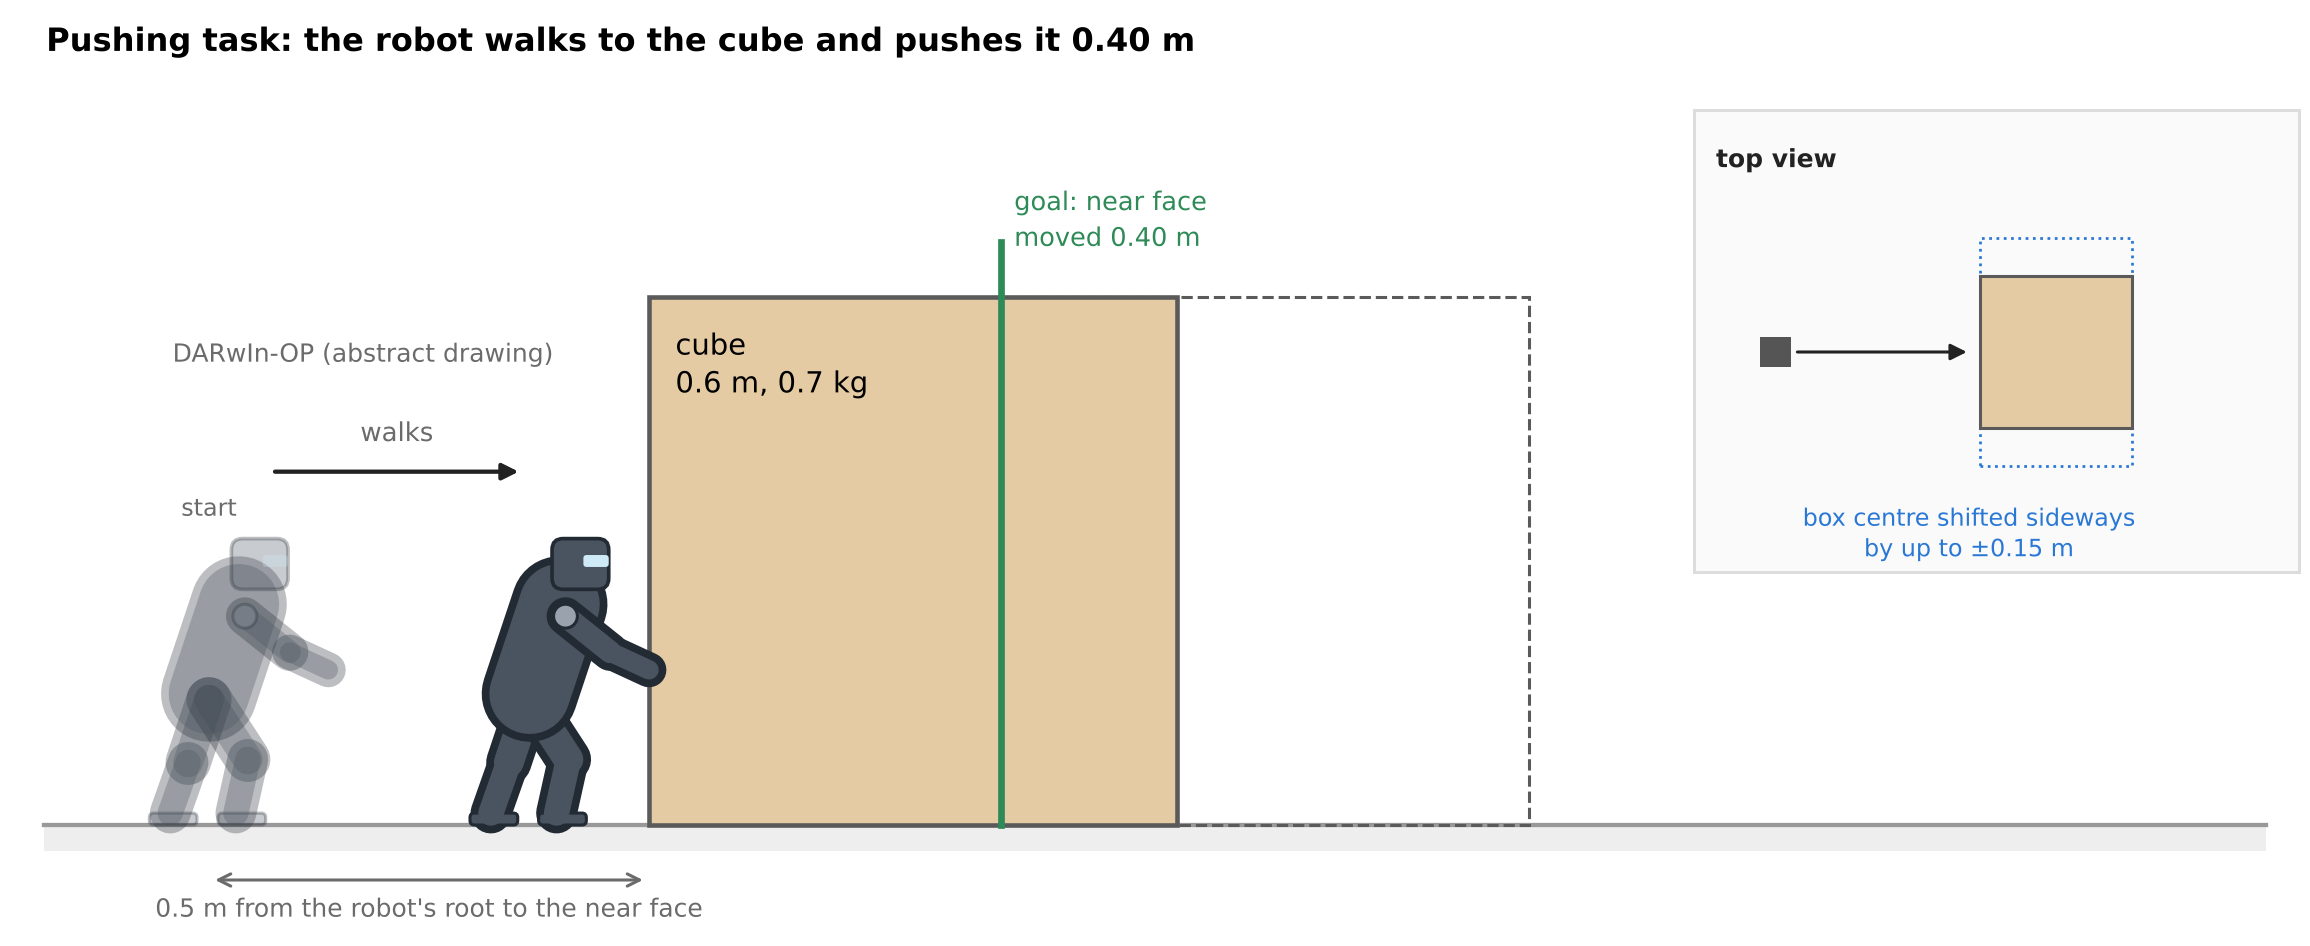
\includegraphics[width=\linewidth]{fig_task.png}
\caption{The pushing task, drawn to scale from the side (an abstract drawing of the DARwIn-OP, which is 0.34~m tall, walks 0.5~m to a 0.6~m cube and pushes it). The inset shows the top view: the box centre is shifted sideways by a fixed offset per episode (up to $\pm0.15$~m in the final queue). Success is the near face of the box moving 0.40~m.}
\label{fig:task}
\end{figure}

\begin{figure}[t]
\centering
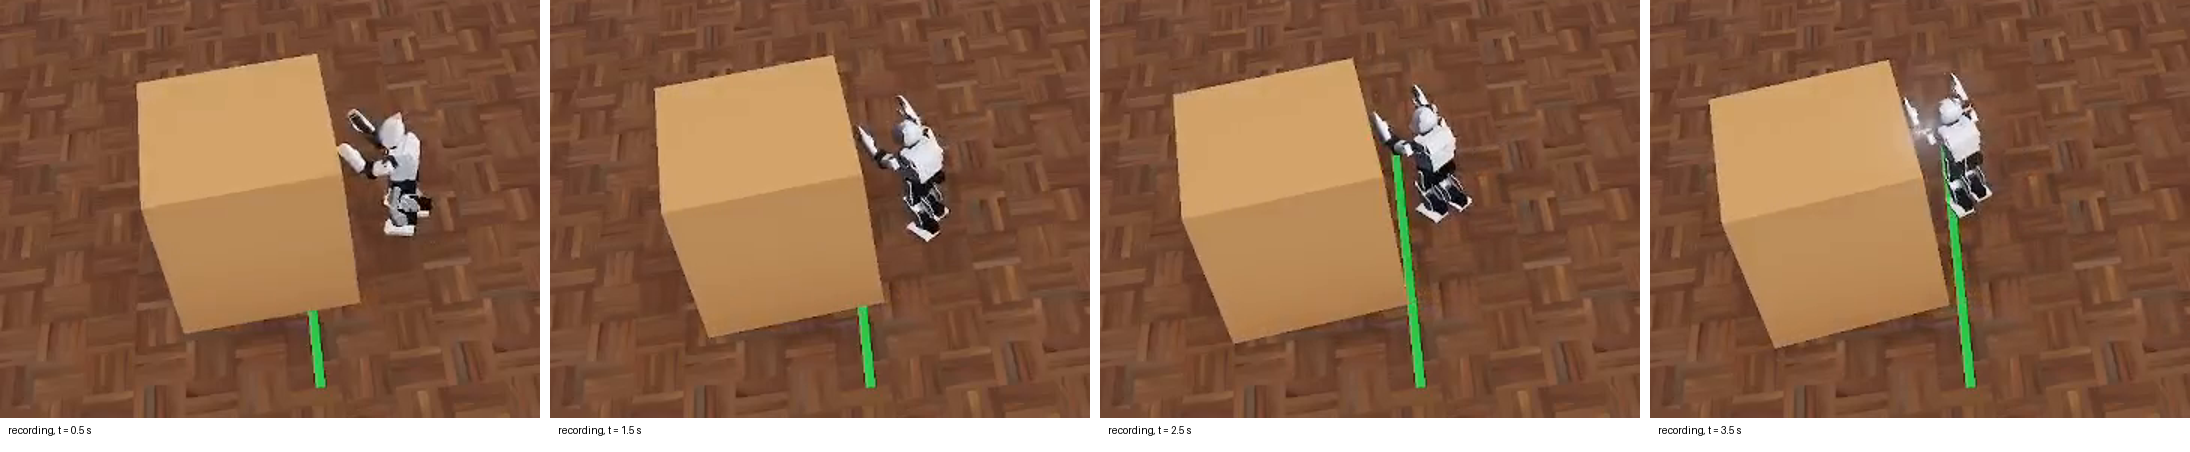
\includegraphics[width=\linewidth]{figs/fig_frames.png}
\caption{Recorded frames of the DARwIn-OP walking to the box and pushing it in Webots, from a screen recording of the open-loop baseline (viewed from above and behind; the green line marks the goal distance).}
\label{fig:frames}
\end{figure}

\begin{figure}[t]
\centering
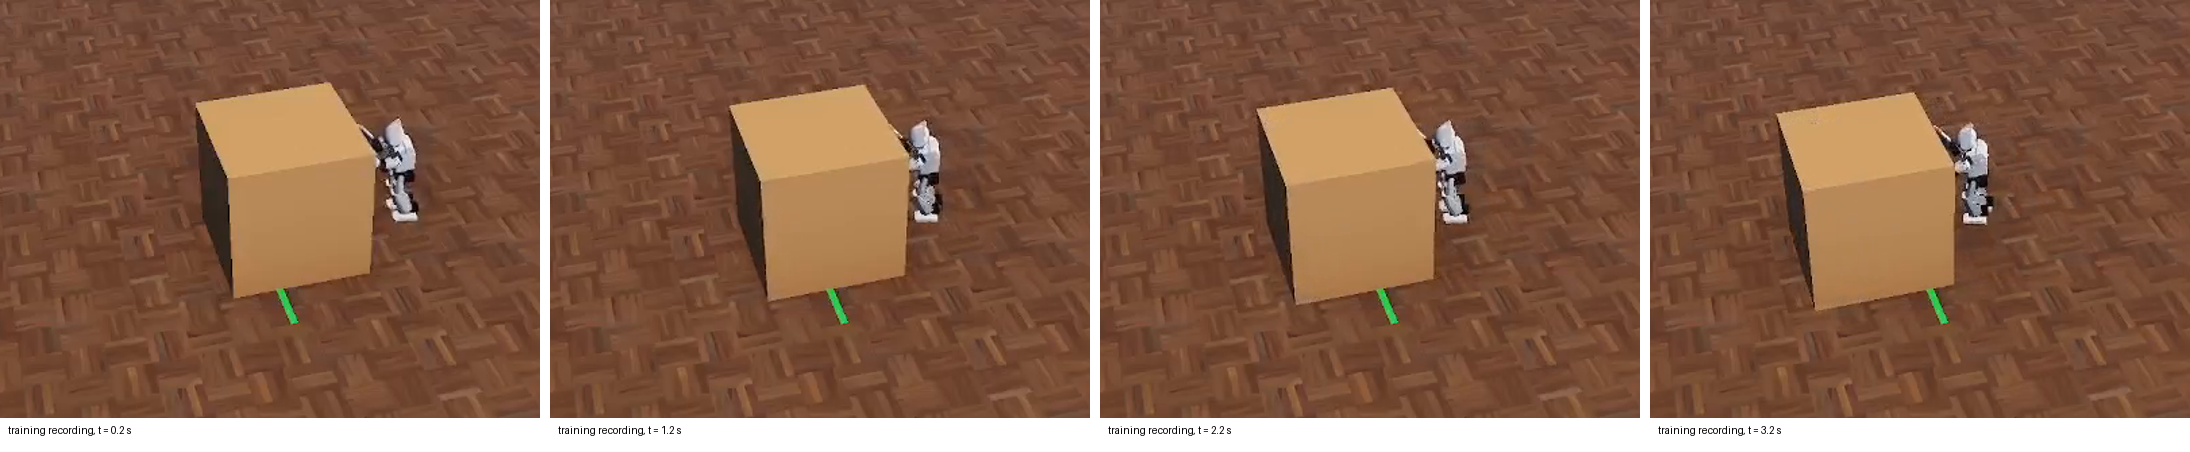
\includegraphics[width=\linewidth]{figs/fig_trained_frames.png}
\caption{Frames from a screen recording of a training run with an H01-subgraph reservoir (readout being trained): the robot stays in contact with the cube and the cube advances toward the green goal line. Training-run candidates are evaluated one after another, so this shows the behaviour qualitatively and is not a success count; success rates are in Tables~\ref{tab:final} and~\ref{tab:pairs}.}
\label{fig:trainedframes}
\end{figure}

\subsection{Training}
Only the readout is trained (Figure~\ref{fig:training}), by an antithetic evolution strategy \citep{salimans2017es}: 16 candidates per generation (8 noise vectors with both signs), centred ranks, step size 0.05, learning rate 0.03, 60 generations. The final trainer picks the checkpoint on 10 separate validation offsets, with the open-loop (zero readout) policy as the first candidate, so a run cannot end below open loop on validation. The first trainer chose checkpoints by a noisy two-episode score and is documented in the results.

\begin{figure}[t]
\centering
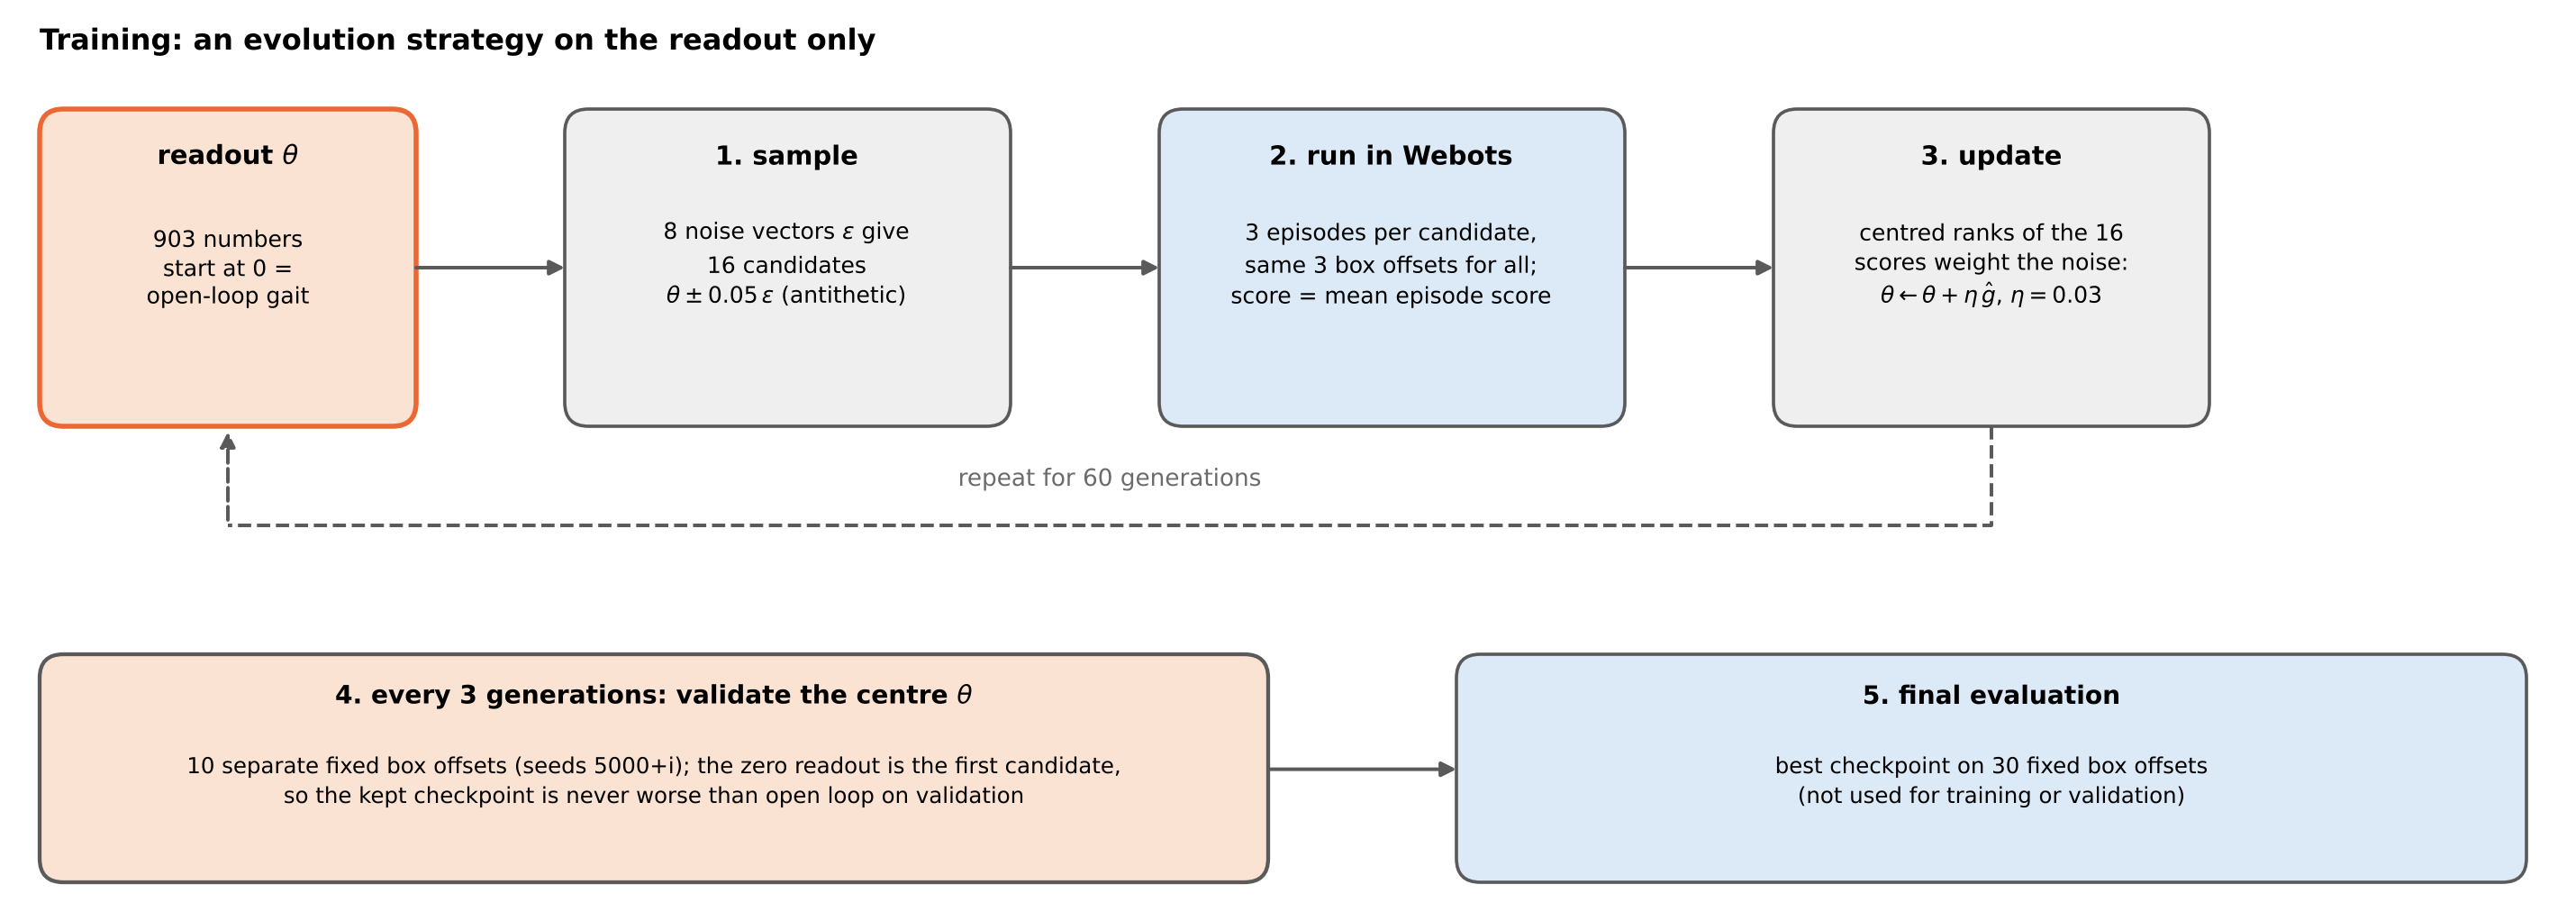
\includegraphics[width=\linewidth]{fig_training.png}
\caption{Training. Each generation perturbs the readout, runs every candidate on three episodes in Webots, and moves the readout along the rank-weighted noise. Every third generation the current readout is validated on separate offsets, and the best validated checkpoint is evaluated once on 30 fixed offsets.}
\label{fig:training}
\end{figure}

\subsection{Controls and Conditions}
Figure~\ref{fig:controls} shows the H01 subgraph beside two of its graph controls. The conditions are:
\begin{itemize}
\item \textbf{H01 data signs:} real wiring, measured signs.
\item \textbf{H01 permute:} real wiring, the same share of inhibitory neurons assigned to random neurons.
\item \textbf{Shuffle:} same neurons, degrees, weights and signs, wiring scrambled by double edge swaps \citep{maslov2002specificity}; \textbf{shuffle + permute} also permutes the signs.
\item \textbf{Random graph:} same size and edge count, random endpoints, shuffled signs.
\item \textbf{ESN:} same size and mean degree, Gaussian weights, one random sign per edge.
\item \textbf{Direct:} linear readout of the 12 inputs, no reservoir (39 trained numbers).
\item \textbf{Bias:} one constant correction, no inputs and no reservoir (3 trained numbers).
\end{itemize}

\begin{figure}[t]
\centering
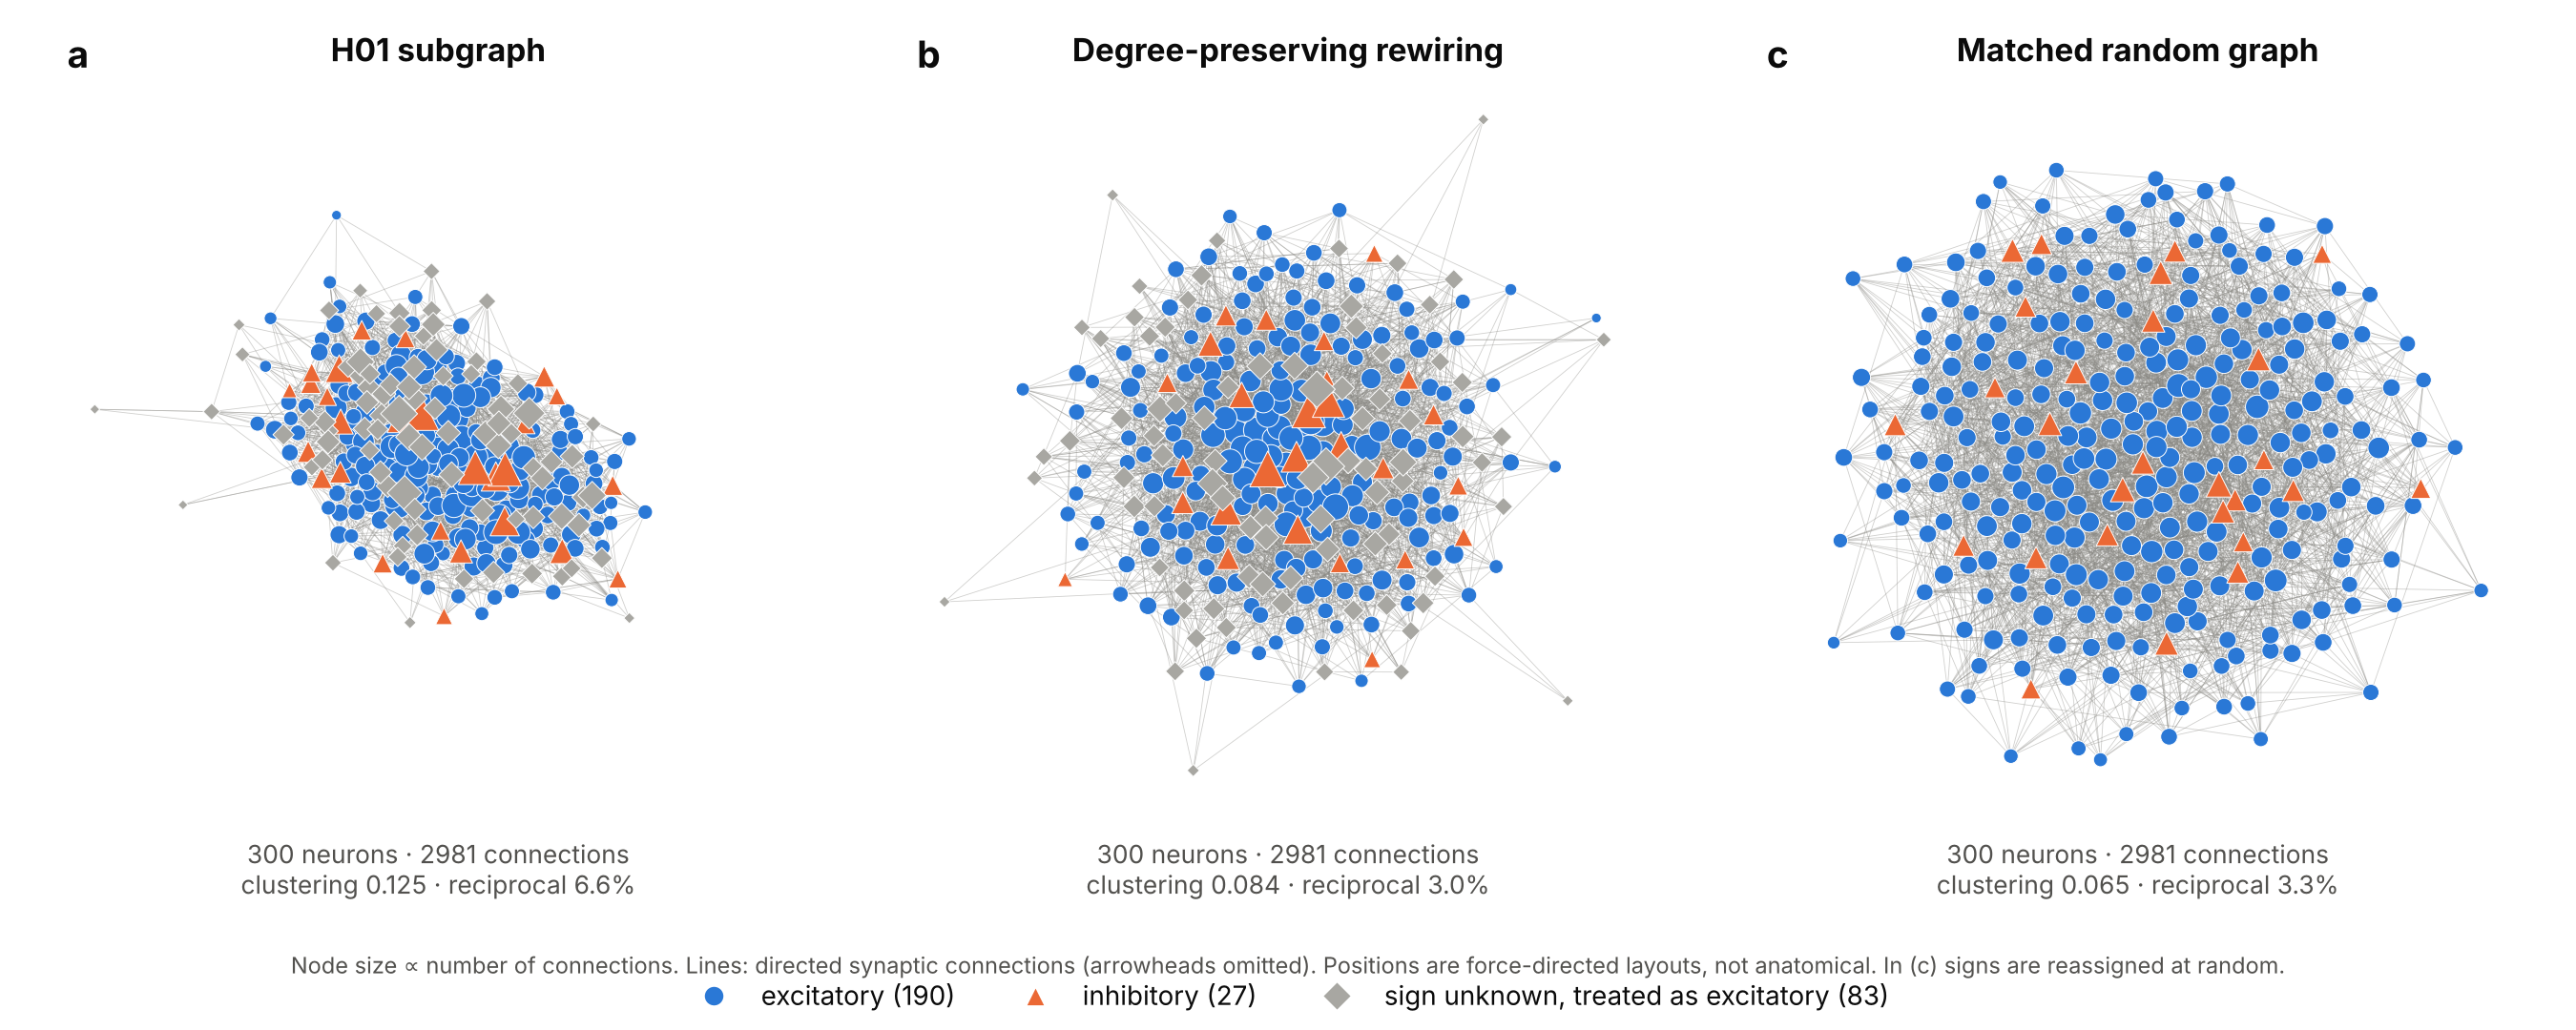
\includegraphics[width=\linewidth]{fig_h01_graph_A_300_s0.png}
\caption{The H01 subgraph s0 (left), its degree-preserving rewiring (middle) and a matched random graph (right). Blue circles: excitatory, orange triangles: inhibitory, grey diamonds: sign unknown.}
\label{fig:controls}
\end{figure}

\section{Experimental Setup}
Three queues were run (Table~\ref{tab:queues}). The v3 difficulty was chosen only from open-loop results, so that open loop succeeded 30--60\% of the time (it succeeded in 10 of 30 episodes). The hypothesis and comparisons were written in the project log before the v3 runs. The controls in v3b (shuffle + permute, direct, bias) were added after v3 and are labelled as such.

\begin{table}[t]
\caption{Experimental Queues}
\label{tab:queues}
\centering
\small
\begin{tabular}{lllllL{0.2\linewidth}}
\toprule
\textbf{Queue} & \textbf{Mass} & \textbf{Offsets} & \textbf{Privileged} & \textbf{Noise} & \textbf{Trainer}\\
\midrule
v1 & 0.5~kg & $\pm0.10$~m & yes & none & first (noisy checkpoint)\\
v2 & 0.5~kg & $\pm0.10$~m & yes & none & validation checkpoint\\
v3, v3b & 0.7~kg & $\pm0.15$~m & no & 0.05 per input & validation checkpoint\\
\bottomrule
\end{tabular}
\end{table}

\section{Results}
In the final queue every trained condition beat open loop, but a constant three-number correction did as well as the best reservoir, and H01 wiring did no better than scrambled wiring.

\subsection{Final Queue (v3 and v3b)}
Open loop at 0.7~kg succeeded in 10 of 30 episodes (33\%, 16 falls, mean score $+0.23$). Trained readouts raised the pooled success rate to between 60\% and 99\% (90 episodes per condition: 30 per subgraph, three subgraphs; Figure~\ref{fig:results}, Table~\ref{tab:final}). The bias-only policy and the ESN each reached 89 of 90, followed by shuffle with permuted signs (87), H01 with permuted signs (85), the direct readout (85), shuffle with measured signs (75), H01 with measured signs (73) and the random graph (54). Falls per episode were 0.00 for bias and direct, 0.01 for ESN, 0.10 for H01 with measured signs and 0.20 for the random graph.

\begin{figure}[t]
\centering
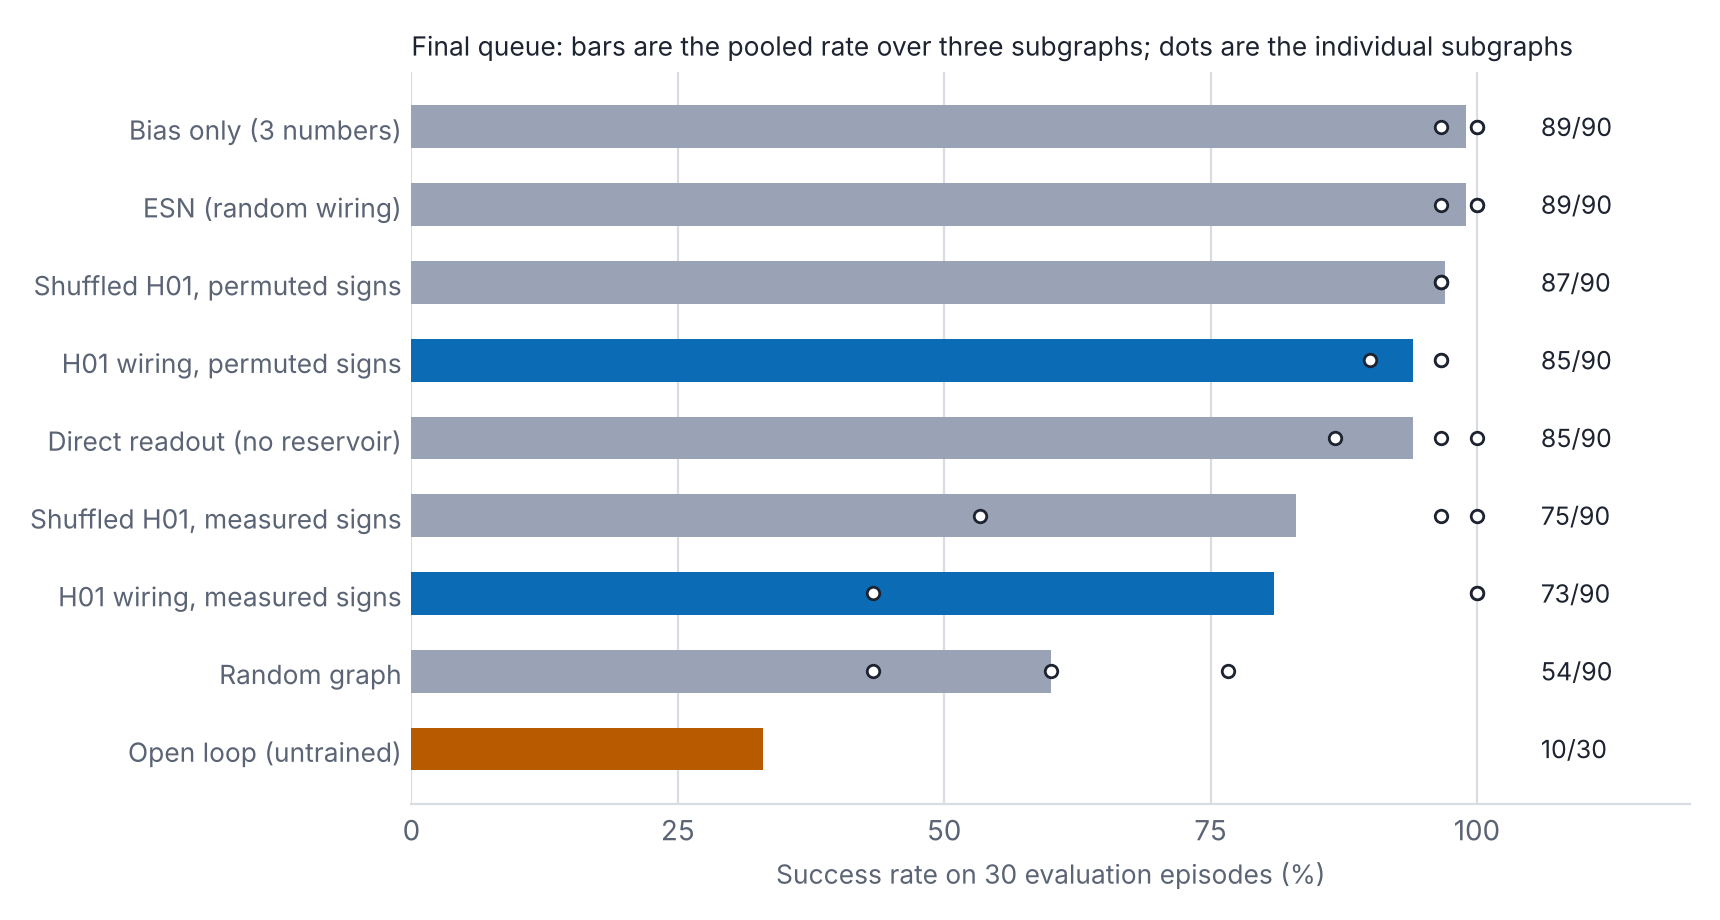
\includegraphics[width=0.9\linewidth]{fig_results.png}
\caption{Final queue (v3 and v3b): pooled success over three subgraphs (bars, successes out of 90) and the three individual subgraphs (dots, 30 episodes each). Blue: H01 wiring; grey: controls; orange: open loop (30 episodes).}
\label{fig:results}
\end{figure}

\begin{table}[t]
\caption{Final Queue: Successes out of 30 per Subgraph}
\label{tab:final}
\centering
\begin{tabular}{lcccc}
\toprule
\textbf{Condition} & \textbf{s0} & \textbf{s1} & \textbf{s2} & \textbf{Pooled (of 90)}\\
\midrule
Bias only (3 numbers)$^{\dagger}$ & 29 & 30 & 30 & 89\\
ESN & 29 & 30 & 30 & 89\\
Shuffle, permuted signs$^{\dagger}$ & 29 & 29 & 29 & 87\\
H01, permuted signs & 29 & 27 & 29 & 85\\
Direct readout$^{\dagger}$ & 29 & 30 & 26 & 85\\
Shuffle, measured signs & 29 & 30 & 16 & 75\\
H01, measured signs & 30 & 30 & 13 & 73\\
Random graph & 18 & 23 & 13 & 54\\
\bottomrule
\end{tabular}

\smallskip
{\footnotesize $^{\dagger}$ added after the main queue (v3b). Open loop: 10 of 30.}
\end{table}

Pairwise comparisons use Fisher's exact test on pooled episodes (Table~\ref{tab:pairs}). They are descriptive, because episodes within a run are not independent and there are only three subgraphs.

\begin{table}[t]
\caption{Pairwise Comparisons (Fisher's Exact Test, Descriptive)}
\label{tab:pairs}
\centering
\begin{tabular}{lcc}
\toprule
\textbf{Comparison} & \textbf{Successes (of 90 each)} & \textbf{$p$}\\
\midrule
H01 data signs vs shuffle (same signs) & 73 vs 75 & 0.85\\
H01 data signs vs random graph & 73 vs 54 & 0.003\\
H01 data signs vs ESN & 73 vs 89 & $<0.0001$\\
H01 data signs vs H01 permuted signs & 73 vs 85 & 0.011\\
H01 permuted signs vs shuffle + permuted signs & 85 vs 87 & 0.72\\
Bias-only vs H01 data signs & 89 vs 73 & $<0.0001$\\
Bias-only vs direct readout & 89 vs 85 & 0.21\\
Bias-only vs ESN & 89 vs 89 & 1.0\\
\bottomrule
\end{tabular}
\end{table}

The pre-registered hypothesis, that H01 wiring with measured signs beats shuffle, random graph, ESN and permuted signs, was therefore not supported: it was better than one control, tied one, and worse than two.

\subsection{Wiring and Signs}
With signs randomised, real and shuffled wiring were indistinguishable (85 vs 87 of 90), so we find no effect of the wiring. Signs mattered more: permuting the measured signs on the same H01 wiring raised success from 73 to 85 of 90. The loss came from the third subgraph, where measured-sign graphs scored 13 and 16 of 30 while permuted-sign graphs scored 29 and 29. This is one subgraph, and our sign labels may be noisy, so we do not read it as a statement about real cortex.

\subsection{Earlier Queues}
Table~\ref{tab:earlier} lists successes out of 30 per subgraph (seeds 0, 1, 2). The first queue used the first trainer, whose checkpoints were chosen by a noisy two-episode score and which sometimes ended below open loop (the 0\% result). The second queue added validation-based checkpoint selection and reached a ceiling. The first-queue H01 result on subgraph 0 (26 of 30) used the last-generation checkpoint, while the other first-queue runs used the best-by-noisy-score checkpoint; we therefore do not compare across the first queue's rows.

\begin{table}[t]
\caption{Earlier Queues: Successes out of 30 per Subgraph (s0, s1, s2)}
\label{tab:earlier}
\centering
\begin{tabular}{lcc}
\toprule
\textbf{Condition} & \textbf{v1 (0.5~kg)} & \textbf{v2 (0.5~kg)}\\
\midrule
H01 data signs & 26, 9, 0 & 29, 20, 28\\
H01 permuted signs & not run & 30, 30, 30\\
H01 random 17\% inhibitory & 20, 28, 15 & 30, 30, 18\\
H01 all excitatory & 1, 5, 3 & not run\\
Shuffle & 3, 8, 0 & 30, 29, 30\\
Random graph & 22, 29, 15 & 30, 30, 29\\
ESN & 22, 28, 28 & 29, 30, 23\\
\bottomrule
\end{tabular}
\end{table}

\subsection{Reliability Notes}
Repeated open-loop evaluations on identical box offsets were not identical (10 of 20 in one run and 5 of 20 in another), so differences of a few episodes are within noise. Part of the third queue's first pass was invalid because the physics world entered a state in which every episode was an instant fall; those eight runs were discarded and redone after we added automatic detection and reload.

\section{Discussion}
In this task, the wiring of a real human cortical subgraph gave no measurable benefit. The task is simple enough that a constant three-number correction solves it, so it cannot yet show whether human-derived structure helps.

\paragraph{What the results suggest.} The gap between open loop (33\%) and the trained conditions comes mostly from retuning the gait for a heavier box, not from sensing or memory. A bias-only policy with no inputs reached 89 of 90, the memoryless direct readout 85, and no reservoir beat either by more than noise. A reservoir can even hurt: the random graph, whose signs are shuffled and whose wiring is random, was the weakest (54 of 90), plausibly because its recurrent activity injects noise into the corrections. Reservoir computing is also known to depend weakly on the exact wiring, which fits our wiring result (real vs scrambled wiring with permuted signs, 85 vs 87 of 90). The sign result is the one structural effect we saw, and it is the least certain: our sign labels rest on an assumption about synapse type, and the inhibitory share in our subgraphs (12--19\%) is below the interneuron share reported for H01 (29\%). A better sign assignment could change this result in either direction.

\paragraph{Next steps.} The main next step is to evaluate the approach on more refined and more difficult tasks, with conditions that change from episode to episode, so that the contribution of connectome-derived wiring can be assessed better. Any such test would keep the matched controls, including the bias-only and direct baselines, and a pre-registered protocol, and would test a network only if the simple baselines fail the task.

\paragraph{What a connectome does and does not give.} It is tempting to read a successful connectome-based controller as a step toward emulating a whole brain, and a failed one as a step away. Our result supports neither claim. A wiring diagram specifies which neurons connect, but not synaptic strengths, neuromodulation, cell-type dynamics or plasticity, and we used only counts of synapses as weights. The H01 volume is roughly a millionth of the volume of a human brain (about 1.05~mm$^3$ against an approximate 1.2 million~mm$^3$; figure to be verified), so a faithful emulation would need orders of magnitude more data and, probably, far more than structure. Whole-brain models of the fly \citep{shiu2024fly} show how far a complete connectome plus simple neuron models can go, and a recent report surveys the gaps \citep{brainemulation2025}. Our experiments make no claim about consciousness or about reconstructing a person from a scan.

\paragraph{Long-term outlook.} The motivation behind this work is a long-term hope, not a result. Suppose that, in some future and by non-destructive means, the full wiring of a human brain could be recorded as a graph, and that a recurrent neural network could be built on that graph. That network could then be given data about the same individual, such as recordings of their voice, videos, writing and other material they produced, to ask whether aspects of their memories or personality could be reconstructed in it. If a general-purpose robot control model could then be attached to such a network, the result would be an embodied system whose core follows one person's wiring. Nothing in our experiments tests this. H01 is a small fragment from surgically removed tissue, no current method records a living human brain at synaptic resolution, and it is unknown whether wiring plus personal data would suffice. We see the present work as a first, controlled step toward a prior question: whether real brain wiring contributes anything to artificial and robotic controllers. We hope this line of work leads to a closer connection between connectomics, artificial intelligence and robotics, starting with simple tasks such as a pushing humanoid and moving on to arms and hands.

\section{Limitations and Reproducibility}\label{sec:limits}
\begin{itemize}
\item \textbf{Scale and sampling.} Three 300-neuron subgraphs of a 16,599-neuron graph, from one cubic millimetre of one brain. Three seeds give little statistical power, and the $p$-values here are descriptive.
\item \textbf{Sign labelling.} Type~1 read as inhibitory is an assumption; 28--31\% of neurons in each subgraph have no sign evidence and default to excitatory.
\item \textbf{Edge weights.} Weights are counts of synapse rows, not measured synaptic strengths.
\item \textbf{One task, one simulator.} A single pushing task in Webots, with some physics instability and non-identical repeated evaluations.
\item \textbf{Protocol history.} The first two queues used four simulator-supplied inputs and an easier box; the final queue removed them. Three controls (shuffle with permuted signs, direct, bias) were added after the main queue, and we label them as such.
\item \textbf{Trainer.} An evolution strategy on 903 readout numbers was unstable; validation-based checkpointing fixed the worst cases but not the variance across runs.
\end{itemize}
We used only the public H01 synapse tables \citep{shapsoncoe2024h01} and did not redistribute them. The code, the derived graph tables, the 100-, 300- and 1,000-neuron subgraph files, the Webots world, the result tables and the project log are planned for release under the MIT licence together with a project page. We thank the H01 authors for releasing the dataset.

\bibliographystyle{plainnat}
\bibliography{refs}

\end{document}
